% ============================================================================
%  第 10 章 拓扑场论中的算子与缺陷
%  译自 Ben-Zvi 讲义第 133–178 页（PDF 页码）
% ============================================================================
\chapter{拓扑场论中的算子与缺陷}\label{ch:10}

\begin{keytakeaways}
本章把“态—算子—缺陷”的量子力学直觉提升为拓扑场论的范畴语言。核心观点是：一个 $n$ 维 TFT 就是从配边范畴到对称幺半范畴的函子 $\mathcal{Z}$——$(n-1)$-维流形给出对象（态空间），$n$ 维配边给出态射；正定向点给 $V$，负定向点给对偶 $V'$，而 1 维 TFT 的公理（求值与余求值满足的“Zorro 之痕”关系）自动蕴含 $V$ 可对偶且有限维。于是“算子”被解释为把正点与负点并置的配边，或等价地解释为两个一维理论之间的界面；界面的复合由“碰撞”配边给出，这为 Hecke 代数、Bernstein 中心与谱分解提供了统一的物理来源。二维 Yang--Mills 理论（有限群）是贯穿全章的模型：边界条件对应表示，局部算子给出交换代数、真空模空间与 B-模型。最后用带奇点的配边假设处理线算子与曲面缺陷，说明高维时局部算子交换、线算子在 3 维为辫状、4 维及以上为对称；并把这套结构落到四维拓扑 Maxwell 理论与几何 Langlands 的 Hecke 对应上。
\end{keytakeaways}

% ============================================================================
\section{态空间}\label{sec:10-1}

\begin{sectionkey}
一维 TFT 就是拓扑量子力学；其配边范畴公理（求值与余求值的 Zorro 关系）恰好等价于“态空间可对偶且有限维”。这为后文“态即边界条件、算子即界面”的整套语言奠定基础。
\end{sectionkey}

一维量子场论就是量子力学。于是我们有一个态空间，即 Hilbert 空间 $H$，并且它被一个可观测量的结合代数 $A$ 所作用。通常 $A$ 由 $H$ 上的全部算子组成。示意性的图像是：$H$ 由某一确定时刻的全部态组成。于是，若有一个态 $\psi\in H_{t_0}$，我们可以在 $t_0$ 之后的某个时刻放置一个算子 $\mathcal{O}$，而经过该算子之后我们得到一个新态 $\mathcal{O}*\psi\in H_{t_1}$。心中要有的图像是：
\begin{equation}\tag{10.1}
\begin{array}{ccc}
\psi_0\in H_{t_0} & \xrightarrow{\ \ \mathcal{O}\ \ } & \mathcal{O}*\psi_0\in H_{t_1}
\end{array}
\end{equation}

这一切在\term{拓扑量子力学}{topological quantum mechanics}中都变得容易得多。

一维 TFT（即拓扑量子力学）是一个对称幺半函子：
\begin{equation}\tag{10.2}
\mathcal{Z}\colon \big(\Bord_1^{\mathrm{or}},\sqcup\big)\longrightarrow\big(\Vect_{\C},\otimes\big).
\end{equation}
$\Bord_1^{\mathrm{or}}$ 的对象是 $0$-流形，但它们是 1-定向的：也就是说，我们为 $n$ 维 TFT 画的所有图像都是 $n$ 维的，因为配边带有 $n$ 维的切向结构。换个说法：你面对的不只是一个 $0$-流形，而是某个\emph{定向} $n$-流形的芽。所以这里可以认为对象是附带一个小的定向区间的 $0$-流形。因此只有两个 1-定向的 $0$-流形：
\begin{equation}\tag{10.3}
\bullet\!\!\longrightarrow \qquad\qquad \longleftarrow\!\!\bullet
\end{equation}
于是函子 $\mathcal{Z}$ 把它们送到两个向量空间：
\begin{equation}\tag{10.4}
\mathcal{Z}\big(\bullet\!\!\longrightarrow\big)=V, \qquad\qquad
\mathcal{Z}\big(\longleftarrow\!\!\bullet\big)=V'.
\end{equation}

\begin{srcrem}{49}
$V$ 最终将是我们的态空间。
\end{srcrem}

现在我们要注意的是，TFT 的公理决定了 $V$ 与 $V'$ 之间的一种密切关系。在 $\Bord_1^{\mathrm{or}}$ 中，从这两个对象的不交并到单位（即空的 $0$-流形 $\varnothing_0$）存在一个自然的态射：
\begin{equation}\tag{10.5}
\big(\bullet\!\!\longrightarrow\big)\;\sqcup\;\big(\longleftarrow\!\!\bullet\big)\;\longrightarrow\;\varnothing_0,
\end{equation}
也就是说，它是：
\diageq{10.6}{0.09\textwidth}{p134_d1.png}
函子 $\mathcal{Z}$ 是对称幺半的，因此它把这个配边送到一个函子，我们称之为求值：
\begin{equation}\tag{10.7}
\mathrm{ev}\colon V\otimes V'\longrightarrow \mathcal{Z}(\varnothing_0)=\C.
\end{equation}
我们还有相反的配边：
\diageq{10.8}{0.09\textwidth}{p134_d2.png}
它给出余求值：
\begin{equation}\tag{10.9}
\mathrm{coev}\colon \C\longrightarrow V\otimes V'.
\end{equation}
这些映射满足一个很好的关系，称为\term{Zorro 之痕}{Mark of Zorro}，因为它来自如下配边：
\diageq{10.10}{0.20\textwidth}{p134_d3.png}
分解这个配边，我们看到函子 $\mathcal{Z}$ 把它送到如下复合：
\begin{equation}\tag{10.11}
V\;\xrightarrow{\ 1\otimes\mathrm{coev}\ }\;V\otimes V'\otimes V\;\xrightarrow{\ \mathrm{ev}\otimes 1\ }\;V,
\end{equation}
\diagram[0.13\textwidth]{p134_d4.png}
其中下图满足交换，即这些映射复合成恒等，因为我们可以把那个配边拉直，而它必须诱导 $V$ 上的恒等映射。

% [Tutor Note: 这里（10.11）下方的小弧箭头即 $\mathrm{id}$；Zorro 关系就是“拉直配边”给出的复合等于恒等。方向务必核对：求值 $V\otimes V'\to\C$、余求值 $\C\to V\otimes V'$，两者顺序不能交换，否则得到的不是对偶公理而是它的转置。]

一旦展开定义，这就是用范畴论的方式说 $V$ 是一个\term{可对偶对象}{dualizable object}，其对偶为 $V'$。这蕴含 $V$ 事实上是有限维的，且 $V'=V^{*}$。

我们可以这样总结：有一个自然的求值映射 $V\otimes V^{*}\to\C$，以及一个自然的恒等映射 $\C\to\End(V)$。而对有限维的 $V$ 有 $V\otimes V^{*}\simeq\End(V)$，于是我们有：
\begin{equation}\tag{10.12}
\begin{array}{ccc}
V\otimes V^{*} & \xrightarrow{\ \ \mathrm{ev}\ \ } & \C\\[5pt]
{\scriptstyle \mathrm{Tr}}\Big\downarrow & & \Big\downarrow{\scriptstyle \mathrm{id}}\\[5pt]
\C & \xrightarrow{\ \ \underset{\mathrm{Tr}(\mathrm{id})=\dim(V)}{\sum e_i\otimes e^i}\ \ } & \End(V)
\end{array}
\end{equation}

% [Tutor Note: （10.12）的四个箭头分别是：上边 $\mathrm{ev}$、左边 $\mathrm{Tr}$（从 $V\otimes V^{*}$ 到 $\C$）、右边 $\mathrm{id}$（从 $\C$ 到 $\End(V)$）、下边 $\sum_i e_i\otimes e^{i}$。注意左右两条竖边的方向不同，容易画反；这里 $e_i$ 与 $e^{i}$ 是对偶基，$\mathrm{Tr}(\mathrm{id})=\dim V$ 正是“对偶配对 + 缩并”给出的维数。]

% ============================================================================
\section{算子}\label{sec:10-2}

\begin{sectionkey}
有限维性把“算子”变成配边：$V\otimes V^{*}=\End(V)$ 对应正点与负点的并置，乘法由把两个这样的对象“焊接”起来的配边给出，作用则由“算子贴着态”的配边给出。
\end{sectionkey}

我们已经看到，$\mathcal{Z}$ 把正定向点送到有限维向量空间 $V$，把负定向点送到对偶空间。这个向量空间 $V$ 就是态空间。现在我们要在这幅图像里找到算子。首先，由于 $V$ 是有限维的，我们有 $V\otimes V^{*}=\End(V)$，它由 $V$ 上的全部算子组成。如果你愿意，这就是 $\mathcal{Z}$ 赋予 $\Bord_1^{\mathrm{or}}$ 的如下对象的值：
\begin{equation}\tag{10.13}
\big(\bullet\!\!\longrightarrow\big)\;\sqcup\;\big(\longleftarrow\!\!\bullet\big)\quad=\quad\bullet\!\!\longrightarrow\!\!\bullet\!\!\longrightarrow
\end{equation}

\begin{srcrem}{50}
眼下我们把这个配边看作式~(10.13) 的左端。下文式~(10.20) 将使用其右端的解读。
\end{srcrem}

代数结构来自如下配边：
\diageq{10.14}{0.20\textwidth}{p135_d3.png}
因为 $A$ 把它送到一个乘法映射：
\begin{equation}\tag{10.15}
\End(V)\otimes\End(V)\longrightarrow \End(V).
\end{equation}
$\End(V)$ 在 $V$ 上的作用来自如下配边：
\diageq{10.16}{0.19\textwidth}{p135_d4.png}
因为 $\mathcal{Z}$ 把它送到一个映射：
\begin{equation}\tag{10.17}
\End(V)\otimes V\longrightarrow V.
\end{equation}

% [Tutor Note: 原文此处写“因为 $A$ 把它送到一个乘法映射”，其中 $A$ 是上一节的可观测量代数；按上下文这里应为 $\mathcal{Z}$，即函子把配边送到乘法映射。记号混用是原稿的笔误，照译并在此指出。]

% ============================================================================
\section{界面}\label{sec:10-3}

\begin{sectionkey}
界面是“两种理论之间的态射”，严格化为双色（蓝/红）配边上的函子。一维情形下，双色场论恰好等价于“一对向量空间 $V,W$ 加上一个映射 $\mathcal{O}\colon W\to V$”，于是态射就是算子、态就是 $\C\to V$ 的界面。
\end{sectionkey}

我们可以用界面的语言同时表述算子与态。设 $V$ 与 $W$ 是两个有限维向量空间。于是可以构造 TFT $\mathcal{Z}_V$ 与 $\mathcal{Z}_W$，其中 $\mathcal{Z}_V$ 把正点送到 $V$，$\mathcal{Z}_W$ 把正点送到 $W$。现在我们来定义 $\mathcal{Z}_V$ 与 $\mathcal{Z}_W$ 之间\term{界面}{interface}（即态射）的概念。

一个界面被编码在\term{双色场论}{bipartite field theory}的概念中，后者是一个函子 $\Bord_1^{\mathrm{or,bi}}\to\Vect$，并满足下面概述的若干性质。范畴 $\Bord_1^{\mathrm{or,bi}}$ 与 $\Bord_1^{\mathrm{or}}$ 相同，只是对象与态射都是\emph{双色流形}。这意味着流形被分解为两部分，我们称之为“蓝”部与“红”部。例如：
\begin{equation}\tag{10.18}
\textcolor{blue}{\rule[0.55ex]{2.6em}{1.1pt}}\!\!\bullet\!\!\textcolor{red}{\rule[0.55ex]{2.6em}{1.1pt}}
\end{equation}
是一个双色 $1$-流形。于是有些双色流形全蓝，有些全红，有些两色兼有。我们对双色场论 $\mathcal{Z}$ 的一项要求是：在完全为红的流形 $R$ 上，$\mathcal{Z}(R)=\mathcal{Z}_V(R)$；在完全为蓝的流形 $B$ 上，$\mathcal{Z}(B)=\mathcal{Z}_W(B)$。然后还有被分解为蓝部与红部的流形。上面的例子给出从蓝色区间到红色区间的一个配边，因此它给出一个映射 $\mathcal{O}\colon W\to V$。所以这个双色流形是我们加进范畴中的一种新的配边。

现在可以证明：这样的双色一维场论对应于一对向量空间 $V,W$，并配有一个映射：
\begin{equation}\tag{10.19}
\mathcal{O}\colon W\longrightarrow V.
\end{equation}
要点是：我们得到一个场论的范畴（态射即界面），它恰好等价于向量空间的范畴。我们要把它想成：$V$ 与 $W$ 沿一个界面相遇，在那里关于 $V$ 的量子力学变成关于 $W$ 的量子力学。

\begin{srcex}{50}
若 $V=W$，则自界面由算子 $\mathcal{O}\in\End(V)$ 标记。其想法是：在两条线相遇的地方，看起来正是 (10.13) 的右端：
\begin{equation}\tag{10.20}
\bullet\!\!\longrightarrow\!\!\bullet\!\!\longrightarrow
\end{equation}
\end{srcex}

同样，一个态 $\psi\in V$ 等同于一个映射 $\C\to V$，它把 $1\mapsto\psi\in V$。于是我们可以把它写成从“平凡”理论 $\mathcal{Z}_{\C}$ 到 $\mathcal{Z}_V$ 的一个界面。我们不去画平凡理论，于是可以把态看成一种新的边界条件：
\begin{equation}\tag{10.21}
\overset{\textstyle V}{\underset{\textstyle \psi}{\bullet\!\!-\!\!-\!\!-\!\!-\!\!-}}
\end{equation}
这里可以想象平凡理论位于 $\psi$ 的左侧。

% [Tutor Note: 界面方向的约定最容易出错：$\mathcal{O}\colon W\to V$ 表示“把蓝（$W$）接到红（$V$）”，与 (10.13) 中“正点 $\sqcup$ 负点”的解读一致；若把 $V$ 与 $W$ 的位置对调，得到的就是 $\mathcal{O}^{T}\colon V^{*}\to W^{*}$ 而不是同一个界面。另外 (10.21) 中“平凡理论在左侧”对应 $\C\to V$ 的箭头方向，画图时不要把它画成 $V\to\C$。]

\begin{flushright}\small 第 20 讲；2021 年 4 月 8 日\end{flushright}

% ============================================================================
\section{二维 TFT}\label{sec:10-4}

\begin{sectionkey}
从一维升到二维，配边成为 2-范畴：对象是 0-流形、1-态射是带 2 维切向结构的区间、2-态射是带角的曲面。二维 TFT 把闭曲面送到数、把 1-流形送到向量空间；而“边界条件”之所以天然构成范畴，是因为存在“界面之间的界面”。
\end{sectionkey}

我们将讨论二维 TFT，着眼于研究算子与缺陷。特别地，我们希望看到 TFT 的内在结构，以及它如何反映在表示论中。

\subsection{基本设定}\label{sec:10-4-1}

设 $\Bord_2^{\mathrm{or}}$ 为定向配边 2-范畴。其对象可以看作带 2 维切空间的 $0$-流形。1-态射是 $0$-流形之间的 $1$-流形配边，我们仍把它视为带有 2 维切空间。我们给配边装备的这个切空间，既是一种记录维数的方式，也是一种指定定向、标架以及其他切向结构的方式。例如，我们可以把一个 $1$-态射画成：
\diageq{10.22}{0.18\textwidth}{p136_d2.png}

2-态射是带角的 $2$-流形。例如，下面是上述 $1$-态射到自身的一个 $2$-态射：
\diageq{10.23}{0.18\textwidth}{p137_d1.png}
我们不久前在图~6.3 中见过同一个配边。

这个 $2$-范畴的重要之处在于：它关于不交并运算是\term{对称幺半}{symmetric monoidal}的，单位由空集 $\varnothing$ 给出。

\begin{srcrem}{51}
配边成族出现，也就是带有分类空间。例如，亏格 $g$ 的闭曲面可以看成从空的 $1$-流形 $\varnothing_1$ 到自身的配边。这些配边构成一个族，由 $\mathrm{B}\,\mathrm{Diff}(\Sigma^{g})$ 给出，而后者等同于亏格 $g$ 曲线的模空间 $\mathcal{M}_g$。
\end{srcrem}

\term{二维 TFT}{two-dimensional TFT}是对称幺半函子：
\begin{equation}\tag{10.24}
\mathcal{Z}\colon\big(\Bord_2^{\mathrm{or}},\sqcup,\varnothing\big)\longrightarrow\big(\mathcal{C},\otimes,1\big).
\end{equation}
这是定义，但我们早已知道二维 TFT 应当给曲面赋数：$\mathcal{Z}(\Sigma)\in\C$；给 $1$-流形赋向量空间 $\mathcal{Z}(N)\in\Vect_{\C}$。这还可以换一种说法。如果我们截断到 $\Bord_{[1,2]}^{\mathrm{or}}$，即不包含角，那么我们实际上应当落到：
\begin{equation}\tag{10.25}
\Bord_{[1,2]}^{\mathrm{or}}\longrightarrow \Vect_{\C}.
\end{equation}
但描述这个截断配边范畴的另一种方式是：空 $0$-流形的自同态
\begin{equation}\tag{10.26}
\End(\varnothing_0),
\end{equation}
也就是说，如果我们想在顶层得到数、在下一层得到向量空间，那么就应当有
\begin{equation}\tag{10.27}
\Vect_{\C}=\End(1_{\C}).
\end{equation}
现在，除这个截断函子之外，要确定 $\mathcal{Z}$ 还需要的额外数据只是一个对象 $\mathcal{Z}(\mathrm{pt})\in\mathcal{C}$。但我们可以用一种典范的方式让这一点更具体。给定任意对象 $C\in\mathcal{C}$，可以附上一个 $\C$-线性范畴：
\begin{equation}\tag{10.28}
\Hom(1_{\C},C).
\end{equation}
我们在一个 $2$-范畴中，所以这确实构成一个范畴；它是 $\C$-线性的，因为可以与单位的自同态作前复合。于是若你有一个函子 $\mathcal{Z}\colon\Bord_2\to\mathcal{C}$，它就提升为：
\begin{equation}\tag{10.29}
\begin{array}{ccc}
\Bord_2 & \longrightarrow & \mathcal{C}\\[3pt]
& \searrow & \Big\downarrow\\[3pt]
& & \mathrm{Cat}_{\C}
\end{array}
\end{equation}
实践中 $\mathcal{C}\to\mathrm{Cat}_{\C}$ 要么是等价，要么是全嵌入。

\begin{srcex}{51}
设 $\mathcal{C}$ 是结合代数的 Morita $2$-范畴。也就是说：对象是结合代数，$A$ 与 $A'$ 之间的 $1$-态射是双模 ${}_A B_{A'}$，$2$-态射是双模之间的映射。它作为 $\C$-线性范畴的全子范畴嵌入，嵌入方式是把一个结合代数送到它的模范畴。
\end{srcex}

% [Tutor Note: 这里 $\mathrm{Cat}_{\C}$ 是 $\C$-线性范畴的 $2$-范畴；(10.29) 的三角形表示“$\Bord_2\to\mathcal{C}$ 可以提升为取值在 $\mathrm{Cat}_{\C}$ 中的函子”，提升的构造就是 (10.28)：$C\mapsto\Hom(1,C)$。注意 $\Hom(1,C)$ 是范畴而不是集合，这是 $2$-范畴与普通范畴的关键差别。]

\subsection{界面与高阶范畴}\label{sec:10-4-2}

现在我们要用 TFT 的语言、而非范畴论的语言来解释这一运算。回忆我们有 TFT 之间\term{界面}{interface}的概念，它是拓扑场论之间的一种“映射”。为此我们使用双色（bipartite）$2$-流形。设 $\mathcal{Z}$ 与 $\mathcal{W}$ 是两个取值在同一范畴中的场论：
\begin{equation}\tag{10.30}
\mathcal{Z},\,\mathcal{W}\colon \Bord_2\longrightarrow \mathcal{C}.
\end{equation}
从 $\mathcal{Z}$ 到 $\mathcal{W}$ 的态射是双色范畴 $\Bord_2^{\mathrm{bi}}$ 上的一个函子。我们不给出正式定义，但一个闭的双色 $2$-流形实际上就是带“红部”与“蓝部”的闭 $2$-流形，如图~10.1。想法是：这个理论通过把 $\mathcal{Z}$ 作用到红色流形上、把 $\mathcal{W}$ 作用到蓝色流形上而给出，此外还有来自这些被分解的流形各被赋予什么的额外信息。我们可以通过记录定向来跟踪它是态射 $\mathcal{Z}\to\mathcal{W}$ 还是 $\mathcal{W}\to\mathcal{Z}$。

\begin{figure}[htbp]
  \centering
  
\includegraphics[width=0.26\textwidth]{figure10-1.png}
  \caption{一个闭的双色 $2$-流形。（原文 p.~138，Figure 10.1）}
  \label{fig:10-1}
\end{figure}

利用某种带奇点的配边假设版本，这些界面对应于映射：
\begin{equation}\tag{10.31}
\mathcal{Z}(\mathrm{pt})\longrightarrow\mathcal{W}(\mathrm{pt}).
\end{equation}
这个态射来自双色配边：
\begin{equation}\tag{10.32}
\text{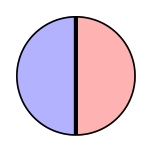
\includegraphics[width=0.045\textwidth]{p138_d2.png}}\;=\;
\textcolor{blue}{\rule[0.55ex]{1.6em}{1.1pt}}\!\!\bullet\!\!\textcolor{red}{\rule[0.55ex]{1.6em}{1.1pt}},
\end{equation}
于是整个结构由 $\mathcal{Z}$、$\mathcal{W}$ 以及理论赋予这个配边的值决定。

设 $C=\mathcal{Z}(\mathrm{pt})$。则 $\Hom(1,C)$ 对应于与 $1$ 相伴的平凡理论和理论 $\mathcal{Z}$ 之间的界面。我们可以把它们画成 $\mathcal{Z}$ 与“空”之间的界面：
\diageq{10.33}{0.16\textwidth}{p138_d3.png}
这就是所谓的 $\mathcal{Z}$ 的\term{边界条件}{boundary condition}或边界理论。

所谓“$\mathcal{C}$ 的对象”（其中 $C\in\mathcal{C}$），按定义指的是底范畴 $\Hom(1,C)$ 的对象。它们等同于态射 $1\to\mathcal{Z}_C$，而后者等同于 $\mathcal{Z}_C$ 的边界理论。$\mathcal{Z}_C$ 的边界理论实际上意味着：我们把函子 $\mathcal{Z}$ 延拓到带一个标记边界分支的 $2$-流形上。也就是说，我仍然看 $2$-流形，但其中一个边界分支标以 $B$，而流形内部标以 $\mathcal{Z}$。

\begin{srcrem}{52}
这是一般构造的一个特例，我们之后会更详细地看到。即：对 TFT $\mathcal{Z}$ 的余维 $k$ 的\term{缺陷理论}{defect theory}意味着把 $\mathcal{Z}$ 从 $n$-流形延拓到带嵌入的、被标记的余维 $k$ 子流形的 $n$-流形上。把这样的延拓记作 $\mathcal{D}_k$，于是我们可以用字母 $\mathcal{D}$ 标记这些子流形。
\end{srcrem}

\begin{figure}[htbp]
  \centering
  
\includegraphics[width=0.24\textwidth]{figure10-2.png}
  \caption{两个界面之间的界面。这是一个带角配边，对应于边界条件 $\mathcal{B},\mathcal{R}\in\Hom(1,\mathcal{Z}(\mathrm{pt}))$ 之间的映射 $\varphi\colon\mathcal{B}\to\mathcal{R}$。（原文 p.~139，Figure 10.2）}
  \label{fig:10-2}
\end{figure}

如果我们在余维 $1$，那么子流形把流形分成两部分，即它是双色流形，于是我们可以用不同的理论标记任一部分。或者我们可以把两部分都标以 $\mathcal{Z}$，这时得到 $\End(\mathcal{Z})$。如果一侧标以平凡理论，就得到边界条件。这里真正发生的是：$0$-球面是不连通的，所以余维 $1$ 子流形的链环不连通，于是每个分支上做什么存在选择。

要点是：二维 TFT $\mathcal{Z}$ 的边界条件构成一个范畴，尽管 $\mathcal{Z}(\mathrm{pt})$ 本身可能不是范畴。任何 $\mathcal{B}\in\Hom(1,\mathcal{Z}(\mathrm{pt}))$ 对应于 $\mathcal{Z}$ 与平凡理论之间的一个界面。作为 $2$-范畴中 $\Hom$ 的对象，意味着它们按定义就构成一个范畴。但这些对象之所以是范畴的对象，其物理原因是存在界面之间的界面，如图~10.2。这对应于边界条件 $\mathcal{B},\mathcal{R}\in\Hom(1,\mathcal{Z}(\mathrm{pt}))$ 之间的映射 $\mathcal{B}\to\mathcal{R}$。

图~10.2 是从如下对象出发的新的带角配边：
\begin{equation}\tag{10.34}
\textcolor{black}{\rule[-1.1ex]{0.8pt}{1.1ex}}\!\!\bullet\!\!\textcolor{red}{\rule[-1.1ex]{0.8pt}{1.1ex}}
\quad\longrightarrow\quad
\textcolor{blue}{\rule[-1.1ex]{0.8pt}{1.1ex}}\!\!\bullet\!\!\textcolor{red}{\rule[-1.1ex]{0.8pt}{1.1ex}}
\end{equation}
这是完全合格的带标记边界的 $1$-流形，于是理论把它们赋予某个向量空间。所以从 $\mathcal{B}$ 到 $\mathcal{R}$ 的界面全体构成一个向量空间。这个向量空间已经是理论的一部分。特别地，它就是如下赋值：
\begin{equation}\tag{10.35}
\mathcal{Z}\big(\textcolor{blue}{\bullet}\!\!\longrightarrow\!\textcolor{red}{\bullet}\big).
\end{equation}
我们可以把这个区间看成奇点的\term{链环}{link}。这些向量空间就是 $\Hom(\mathcal{B},\mathcal{R})$。配边：
\diageq{10.36}{0.17\textwidth}{p139_d2.png}
或等价的“马裤对”（pair of chaps）配边：
\diageq{10.37}{0.20\textwidth}{p140_d1.png}
二者都诱导复合映射：
\begin{equation}\tag{10.38}
\Hom(\mathcal{B},\mathcal{G})\otimes\Hom(\mathcal{G},\mathcal{R})\longrightarrow\Hom(\mathcal{B},\mathcal{R}).
\end{equation}
因此这些向量空间像范畴中的态射一样复合。

同样的想法在任意维数都成立。对 $n$ 维 TFT，我们可以构造边界理论的 $(n-1)$-范畴，其中对象是边界条件，$1$-态射是边界条件之间的界面，$2$-态射是界面之间的界面，如此一直进行到第 $(n-1)$ 层，因为理论是 $n$ 维的。

% [Tutor Note: 这里是全章第一个容易混淆的地方：$\mathcal{Z}(\mathrm{pt})$ 可能不是范畴，但它的“边界条件”却按定义构成范畴 $\Hom(1,\mathcal{Z}(\mathrm{pt}))$。“界面之间的界面”之所以存在，是因为余维 1 子流形的链环是 $S^{0}$（两个点），两个端点可以各自独立地选择边界条件。(10.34) 中的颜色正是标记两个端点所接的边界条件，复合则由 (10.37) 的“马裤对”配边给出。]

\subsection{有限群的二维 Yang--Mills 理论}\label{sec:10-4-3}

这也称为无扭转的 \term{Dijkgraaf--Witten 理论}{untwisted Dijkgraaf--Witten theory}。设 $G$ 是有限群。于是我们定义一个二维 TFT：
\begin{equation}\tag{10.39}
\mathcal{Z}_G\colon \Bord_2^{\mathrm{or}}\longrightarrow \mathrm{Cat}_{\C},
\end{equation}
其构造方式是把流形上 $G$-局部系统的空间线性化。

这将是一个\term{拉格朗日场论}{Lagrangian field theory}，意思如下。我们有这个配边范畴 $\Bord_2^{\mathrm{or}}$，然后从它出发有一个场的构造，取值落在某种几何对象（如群胚）中，然后我们再线性化（例如取层），落到 $\mathrm{Cat}_{\C}$ 中：
\begin{equation}\tag{10.40}
\begin{array}{ccccc}
\Bord_2^{\mathrm{or}} & \xrightarrow{\ F\ } & \mathrm{Grpd} & \xrightarrow{\ \mathrm{Shv}\ } & \mathrm{Cat}_{\C}\\[4pt]
& \searrow & & \swarrow & \\
& & \scriptstyle \mathcal{Z}=\mathrm{Shv}(F(-)) & &
\end{array}
\end{equation}
若 $\Sigma$ 是闭的 $2$-流形，则 $\mathcal{Z}_G(\Sigma)$ 是 $\Sigma$ 上 $G$-局部系统的个数。回忆 $G$-局部系统由下式给出：
\begin{equation}\tag{10.41}
\Loc_G\Sigma=\{\pi_1\Sigma\to G\}\big/\!\sim,
\end{equation}
但当我们数它们时，要按自同构加权：
\begin{equation}\tag{10.42}
\mathcal{Z}_G(\Sigma)=\sum_{P\in\Loc_G\Sigma}\frac{1}{|\Aut(P)|}.
\end{equation}
若 $N^1$ 是 $1$-流形，我们赋予：
\begin{equation}\tag{10.43}
\mathcal{Z}_G\big(N^1\big)=\C\big[\Loc_G N\big],
\end{equation}
这里我们只是把 $\Loc_G N$ 看作有限群胚。若 $P^0$ 是 $0$-流形，则
\begin{equation}\tag{10.44}
\mathcal{Z}_G\big(P^0\big)=\Vect\big(\Loc_G P^0\big).
\end{equation}

例如，
\begin{equation}\tag{10.45}
\mathcal{Z}_G\big(S^1\big)=\C\big[\Loc_G S^1\big]=\C\left[\frac{G}{G}\right],
\end{equation}
它们是\emph{类函数}。对零维流形 $\mathrm{pt}$ 我们有：
\begin{align}
\mathcal{Z}_G(\mathrm{pt})&=\Vect\big(\Loc_G(\mathrm{pt})\big)\tag{10.46}\\
&=\Vect\big(\mathrm{pt}/G\big)\tag{10.47}\\
&=\Rep(G).\tag{10.48}
\end{align}
设 $M$ 是从 $N_{\mathrm{in}}$ 到 $N_{\mathrm{out}}$ 的配边。取 $\Loc_G$ 给出群胚的对应（span，即双拉回图）：
\begin{equation}\tag{10.49}
\begin{array}{ccc}
& \Loc_G M &\\[4pt]
\swarrow & & \searrow\\[4pt]
\Loc_G N_{\mathrm{in}} & & \Loc_G N_{\mathrm{out}}
\end{array}
\end{equation}
在这些群胚上取函数给出：
\begin{equation}\tag{10.50}
\pi_{\mathrm{out},*}\pi_{\mathrm{in}}^{*}\colon \C\big[\Loc_G N_{\mathrm{in}}\big]\longrightarrow\C\big[\Loc_G N_{\mathrm{out}}\big].
\end{equation}
这就是流形之间的配边如何变成相应函数空间之间的映射。

\textbf{问题 4.} 如何看出 $G$ 的\emph{表示}？

抽象地说我们有 $\mathcal{Z}_G(\mathrm{pt})=\Rep(G)$。于是表示 $V\in\Rep(G)$ 等同于 $\mathcal{Z}_G(\mathrm{pt})$ 的一个对象，而后者等同于一个函子 $\Vect\to\Rep(G)$，它把 $\C$ 送到 $V$。也就是说，这是从平凡理论到 $\mathcal{Z}_G$ 的一个界面，即 $\mathcal{Z}_G$ 的一个边界条件。

但这与“带颜色的边界”有什么关系？给定 $G$ 的表示 $V$（我们把它想成“红色”），我们可以把 $\mathcal{Z}_G$ 延拓到带红色边界分支的流形上。例如，我们有一种新的 $1$-配边：
\begin{equation}\tag{10.51}
\textcolor{red}{\bullet}\!\!-\!\!-\!\!-\!\bullet
\end{equation}
它对应于对象 $V\in\mathcal{Z}_G(\mathrm{pt})$。

同样，一个边界分支被标为红色的柱面给出 $\mathcal{Z}_G(S^1)$ 的一个元素。这个元素恰好是 $V$ 的\term{特征}{character}：$\chi_V\in\C\big[G/G\big]$。

物理的解释如下。$V\in\Rep(G)$ 当然是一个向量空间，所以我们可以把它看成定义拓扑量子力学理论的态空间。但把它变成表示，意味着我们把一维理论\emph{耦合}到了体（bulk）规范理论 $\mathcal{Z}_G$ 上。所以我们考虑的是一个量子力学理论，它生活在某些 $1$-流形上，而这些 $1$-流形是某个体的边界，在那个体上我们有理论 $\mathcal{Z}_G$。

\begin{srcex}{52}
回忆正则表示 $\mathrm{Reg}=\C[G]$。它对应于 $\mathcal{Z}_G$ 的 Dirichlet 边界条件。平凡表示 $\C$ 对应于 Neumann 边界条件。
\end{srcex}

我们对这些边界条件能做的主要事情，是讨论它们之间的界面。于是，如果我有一个表示 $V$，以及一个蓝色的表示 $W$，那么一个界面：
\diageq{10.52}{0.15\textwidth}{p142_d1.png}
是 $\mathcal{Z}_G$ 赋予该奇点的链环的那个向量空间的一个元素：
\begin{equation}\tag{10.53}
\mathcal{Z}\big(\textcolor{red}{\bullet}\!\!-\!\!-\!\!-\!\textcolor{blue}{\bullet}\big)=\Hom_{\Rep(G)}(V,W).
\end{equation}
而复合由这种缺陷的碰撞、也就是“马裤对”配边来实现。

现在我们将用场的语言来写边界条件的范畴。带有 $G$ 作用的集合是 $G$ 的表示的一个简单来源，因为 $G\curvearrowright X$ 蕴含 $\C[X]$ 是 $G$-表示。于是我们可以认为边界条件由 $G\curvearrowright X$ 指定，而这里我们暗中把它与表示 $\C[X]$ 联系起来。在体内部我们有 $\Loc_G$，所以总的场空间由 $G$-局部系统连同边界上相伴 $X$-丛的一个截面组成。也就是说，我们把整个曲面映射到 $\mathrm{pt}/G$（这就是为什么得到 $\Loc_G$），然后在标以 $X$ 的边界上，把这个映射提升到 $X/G$：
\begin{equation}\tag{10.54}
\begin{array}{ccc}
& & X/G\\[4pt]
& \nearrow & \Big\downarrow\\[4pt]
\partial\Sigma & \xrightarrow{\qquad} & \mathrm{pt}/G
\end{array}
\end{equation}

\begin{srcex}{53}
若 $X=G$（于是我们考虑的是正则表示），则 $X/G=\mathrm{pt}$，我们考虑的是 $G$-局部系统连同边界上的一个平凡化，这就是 Dirichlet 边界条件。
\end{srcex}

\begin{flushright}\small（原稿批注：transition。）\end{flushright}

% [Tutor Note: 本节有三处约定需要记牢。(1) 边界条件的颜色：红/蓝对应 $V$/$W$，界面方向是 $\Hom_{\Rep(G)}(V,W)$，即 (10.53) 的 $\mathcal{Z}(\text{红}\to\text{蓝})$，不要与反方向的 $\Hom(W,V)$ 混淆。(2) 正则表示 $\C[G]$ 对应 Dirichlet 边界条件、平凡表示 $\C$ 对应 Neumann，这与下一节 $X=G/1$ 对 Dirichlet、$X=\mathrm{pt}=G/G$ 对 Neumann 的“几何”说法是同一件事。(3) 柱面上的元素是特征 $\chi_V$，而不是维数 $\dim V$；维数只在把柱面闭合（再取迹）时出现。]

\begin{flushright}\small 第 21 讲；2021 年 4 月 13 日\end{flushright}

% ============================================================================
\section{拉格朗日理论中的边界条件}\label{sec:10-5}

\begin{sectionkey}
在拉格朗日理论中，边界条件不是“约束”而是“额外结构”：要求到目标 $Y$ 的映射在边界上提升到某个 $Z\to Y$。对有限群 Yang--Mills，$Z\to Y$ 等价于一个 $G$-空间，于是边界条件就是表示；边界条件之间的界面则是 $H\backslash G/K$ 型的双陪集，其复合给出 Hecke 代数。
\end{sectionkey}

基本的图像是：我们考虑从某个时空 $\Sigma$ 到某个目标 $Y$ 的映射理论，即场是映射，而我们对它作线性化。我们可能允许 $\Sigma$ 有边界，然后可以在边界上施加条件。例如，若选取某个子流形 $Z\subset Y$，我们可能要求映射 $\psi\colon\Sigma\to Y$ 把 $\partial\Sigma$ 送到 $Z$：
\begin{equation}\tag{10.55}
\varphi|_{\partial\sigma}\subset Z.
\end{equation}

\begin{srcrem}{53}
为了表述这个问题，我们并不需要 $Z$ 是子流形。我们可以只取某个映射 $Z\to Y$，并要求到 $Y$ 的映射在边界上提升到 $Z$：
\begin{equation}\tag{10.56}
\begin{array}{ccc}
\partial\Sigma & \longrightarrow & Z\\[4pt]
\downarrow & & \downarrow\\[4pt]
\Sigma & \xrightarrow{\ \ \varphi\ \ } & Y
\end{array}
\end{equation}
\end{srcrem}

于是现在我们既有 $\varphi\colon\Sigma\to Y$，又有 $\varphi|_{\partial\Sigma}$ 提升到 $Z$ 的数据：
\begin{equation}\tag{10.57}
\widetilde{\varphi}_{\partial}\colon\partial\Sigma\longrightarrow Z.
\end{equation}

要点是：我们并不是真的在施加一个条件，而是在添加一个映射的额外结构。因此，\emph{边界理论}（boundary theory）可能是比“边界条件”更好的名字。

回忆我们当时研究的是有限群的 Yang--Mills 理论。这是目标为 $Y=\mathrm{pt}/G$ 的理论。于是映射 $\varphi\colon\Sigma\to\mathrm{pt}/G$ 给出 $\Sigma$ 上的一个 $G$-丛。对有限群 $G$，这意味着我们得到的正是 $\Loc_G\Sigma$。

给出一个映射 $Z\to Y=\mathrm{pt}/G$，等价于给出空间 $G\curvearrowright X$。具体地说，对于一个映射：
\begin{equation}\tag{10.58}
\begin{array}{c}
Z\\[-2pt]
\downarrow\\[-2pt]
Y=\mathrm{pt}/G
\end{array}
\end{equation}
我们可以把 $G$-空间 $G\curvearrowright X$ 构造为纤维积：
\begin{equation}\tag{10.59}
\begin{array}{ccc}
X & \longrightarrow & Z\\[4pt]
\downarrow & & \downarrow\\[4pt]
\mathrm{pt} & \longrightarrow & Y=\mathrm{pt}/G
\end{array}
\end{equation}
反之，从一个 $G$-空间 $G\curvearrowright X$ 出发，我们可以构造：
\begin{equation}\tag{10.60}
\begin{array}{c}
Z=X/G\\[-2pt]
\downarrow\\[-2pt]
Y=\mathrm{pt}/G
\end{array}
\end{equation}
因此，一个 $G$-空间 $G\curvearrowright X$ 给出一个边界理论。在此之前我们有
\begin{equation}\tag{10.61}
\Loc_G(\Sigma)=\{\Sigma\to\mathrm{pt}/G\}.
\end{equation}
当 $\Sigma$ 有边界时，我们就可以要求提升到：
\begin{equation}\tag{10.62}
\begin{array}{ccc}
\partial\Sigma & \xrightarrow{\ \ \widetilde{\varphi}_{\partial}\ \ } & X/G\\[4pt]
\downarrow & & \downarrow\\[4pt]
\Sigma & \xrightarrow{\ \ \varphi\ \ } & \mathrm{pt}/G
\end{array}
\end{equation}
这些构成：
\begin{equation}\tag{10.63}
\Loc_G^{X}(\Sigma,\partial\Sigma).
\end{equation}
具体地说，$\varphi$ 对应于一个 $G$-丛：
\begin{equation}\tag{10.64}
\begin{array}{c}
\mathcal{P}\\[2pt]
{\scriptstyle G}\downarrow\\[2pt]
\Sigma
\end{array}
\end{equation}
而提升 $\widetilde{\varphi}_{\partial}$ 的数据等价于相伴 $X$-丛的一个截面：
\begin{equation}\tag{10.65}
\begin{array}{c}
P|_{\partial\Sigma}\times^{G}X\\[2pt]
\downarrow\\[2pt]
\partial\Sigma
\end{array}
\end{equation}
其纤维看起来像 $X$，而过渡数据由作用 $G\curvearrowright X$ 给出。

\textbf{练习 1.} 证明：提升到 $X/G$ 的数据等价于这个相伴 $X$-丛的一个截面。

这个数据也等价于一个 $G$-等变映射 $\mathcal{P}|_{\partial\Sigma}\to X$。

\begin{srcrem}{54}
用物理学的话说，我们是在边界上把 $\Sigma$-模型耦合到 $X$、而体内是 $G$-规范理论。也就是说，在边界上我们有一个低一维的、映入 $X$ 的映射理论，在内部我们有一个关于 $G$-丛的理论，然后把它们拼在一起构造这个耦合理论的场。
\end{srcrem}

\begin{srcex}{54}
若 $X=G/H$，则相伴 $X$-丛的截面 $\mathcal{P}\times^{G}X=\mathcal{P}\times^{G}G/H$ 等同于把 $\mathcal{P}$ 从 $G$ 约化到 $H$。也就是说，这等同于把 $\mathcal{P}$ 写成由某个 $H$-丛诱导出来的。

例如若 $X=G=G/1$，则相伴 $X$-丛的截面等同于 $\mathcal{P}|_{\partial\Sigma}$ 的一个平凡化。这是 Dirichlet 边界条件的规范理论版本。回忆在我们的二维 TFT $\mathcal{Z}_G$（Yang--Mills 理论）中，边界条件对应于 $\Rep(G)$。具体地，一个 $G$-空间给出表示 $\C[X]$。与 $X=G/1$ 相伴的边界条件对应于正则表示 $\C[G]\in\Rep(G)$。

另一个极端是 $X=\mathrm{pt}=G/G$。这就是所谓的 Neumann 条件。它对应于平凡表示 $\C\in\Rep(G)$。
\end{srcex}

% [Tutor Note: (10.55) 中原文写作 $\varphi|_{\partial\sigma}\subset Z$，下标是小写 $\sigma$，而全章其余地方用 $\Sigma$；这应是原稿笔误，照译于此指出。另一个更实质的易错点是“边界条件”的措辞：如作者强调的，它其实是“把映射在边界上提升到 $Z$”的额外结构，而不是对场施加的等式约束；这正是 $X=G/1$ 给出 Dirichlet（平凡化）、$X=\mathrm{pt}$ 给出 Neumann（无附加数据）的原因。]

\subsection{边界条件之间的界面}\label{sec:10-5-1}

现在我们来考虑边界条件之间的界面，在线性化之后它们将对应于表示之间的映射。考虑由表示 $V$ 与 $W$ 给出的两个边界条件。假设 $V$ 来自 $G$-空间 $X_1$，而 $W$ 来自 $G$-空间 $X_2$。那么考虑它们之间的一个界面：
\diageq{10.66}{0.13\textwidth}{p144_d1.png}
这个界面被什么标记？我们已经看到它对应于表示的一个映射；但用 $G$-空间 $X_i$ 来说，我们构造纤维积：
\begin{equation}\tag{10.67}
\begin{array}{ccc}
T & \longrightarrow & X_2/G\\[4pt]
\downarrow & & \downarrow\\[4pt]
X_1/G & \longrightarrow & \mathrm{pt}/G
\end{array}
\end{equation}
而这个界面由如下东西标记：
\diageq{10.68}{0.13\textwidth}{p144_d3.png}

这正是放在这里的自然之物：如果我们在边界的一部分上有一个到 $X_1$ 的提升，在边界的另一部分上有一个到 $X_2$ 的提升，那么在重叠处我们应当提升到某个映射到 $T$ 的东西。

\begin{srcex}{55}
若 $X_1=G/H$ 且 $X_2=G/K$，则 $X/G=\mathrm{pt}/H$ 且 $X_2/G=\mathrm{pt}/K$，于是纤维积为：
\begin{equation}\tag{10.69}
\begin{array}{ccc}
H\backslash G/K & \longrightarrow & \mathrm{pt}/K\\[4pt]
\downarrow & & \downarrow\\[4pt]
\mathrm{pt}/H & \longrightarrow & \mathrm{pt}/G
\end{array}
\end{equation}
也就是说：如果我们在 $\Sigma$ 上有一个 $G$-丛，它在边界的一部分上把结构群从 $G$ 约化到 $H$，在边界的另一部分上从 $G$ 约化到 $K$，那么在重叠处我们就同时约化到 $H$ 和 $K$，而这些由到 $H\backslash G/K$ 的映射给出。也就是说，$\mathrm{pt}/H$ 与 $\mathrm{pt}/K$ 之间的几何/拉格朗日界面由 $H\backslash G/K$ 给出。自界面由 $K\backslash G/K$ 给出。

形象地说我们有：
\begin{equation}\tag{10.70}
H\backslash G/K=\begin{array}{ccc}
& \mathrm{pt}/G &\\[-5pt]
& \bullet &\\[3pt]
\bullet & \longrightarrow & \bullet\\[-6pt]
\mathrm{pt}/H & & \mathrm{pt}/K
\end{array}
\end{equation}
也就是说，我们在内部有一个 $G$-丛，它在一个端点约化为 $H$-丛、在另一个端点约化为 $K$-丛。所有这类丛构成的空间就是 $H\backslash G/K$。
\end{srcex}

\textbf{问题 5.} 这幅图像如何与我们之前的图像联系起来？

我们此前已经稍微看到了这一点，基本想法是：它们通过“从奇点过渡到其链环”联系起来。链环是奇点的一个小管状邻域的边界。所以在这个例子里，我们研究的是 $\mathrm{pt}/H$ 与 $\mathrm{pt}/K$ 之间的界面，而链环是那个绿色区间：
% 校订注：原译文只嵌左侧半圆盘裁件、以中文括注代替右侧绿色区间，且裁件右缘把 pt/G 截成 pt。
% 2026-11-19 由原 PDF p.145 以 400 dpi 重裁整幅（左盘 ≃ 右区间），改为单张图示方程。
\diageq{10.71}{0.46\textwidth}{p145_d2.png}

\subsection{边界条件之间界面的复合}\label{sec:10-5-2}

现在我们要理解界面的复合。Hecke 代数正是以这种方式从物理中获得代数结构的。

物理的图像（称为\term{算子乘积展开}{operator product expansion}，简称 OPE）是：我们有两个界面，但从远处看它看起来像两个界面：
\begin{equation}\tag{10.72}
\text{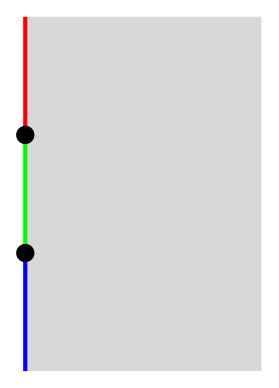
\includegraphics[width=0.11\textwidth]{p146_d1.png}}\quad\simeq\quad
\text{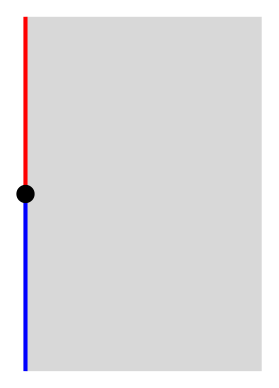
\includegraphics[width=0.11\textwidth]{p146_d2.png}},
\end{equation}
形式上我们可以按 (10.71) 附近的讨论取奇点的链环，得到：
\begin{equation}\tag{10.73}
\text{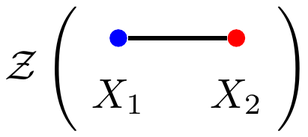
\includegraphics[width=0.22\textwidth]{p146_d3.png}}\;=\;\Hom(X_1,X_2).
\end{equation}
然后“马裤对”配边：
\diageq{10.74}{0.17\textwidth}{p146_d4.png}
诱导出复合映射：
\begin{equation}\tag{10.75}
\Hom(X_1,X_2)\otimes\Hom(X_2,X_3)\longrightarrow\Hom(X_1,X_3).
\end{equation}
Hecke 代数出现在我们考虑三个边界上都约化到 $K$ 的 $G$-丛时：
\begin{equation}\tag{10.76}
\text{（与 (10.74) 相同的“马裤对”配边，只是三个边界 }K,K,K\text{ 都被标以 }K\text{）}
\end{equation}
这幅图给出乘法映射：
\begin{equation}\tag{10.77}
\C[K\backslash G/K]\otimes\C[K\backslash G/K]\longrightarrow\C[K\backslash G/K].
\end{equation}
这就是 Hecke 代数的物理再解释。

\begin{srcex}{56}
若 $K=1$（Dirichlet 边界条件），则 $K\backslash G/K=G$，而这幅图恢复出群代数 $\C G$。
\end{srcex}

\begin{srcex}{57}
若 $K=G$（Neumann 边界条件），则场空间是 $\mathrm{pt}/G$。但 $\C[\mathrm{pt}/G]=\C$，于是 Hecke 代数是 $\End_{\Rep}(\C)=\C$。
\end{srcex}

% [Tutor Note: Example 55 中原文写“$X/G=\mathrm{pt}/H$”，按上下文应为 $X_1/G=\mathrm{pt}/H$（$X_2/G=\mathrm{pt}/K$ 才是另一个），这是原稿的指标笔误，照译并指出。另需注意 $K\backslash G/K$ 的复合正是卷积：$K=1$ 时退化为群代数 $\C G$，$K=G$ 时退化为 $\C$，这两个极端之间才是真正非交换的 Hecke 代数。此外 (10.76) 原图为与 (10.74) 同样的“马裤对”配边，仅把三个边界标号都改成 $K$。]

对向量空间 $V$，有 $\End(V)\curvearrowright V$。若 $V\in\Rep(G)$，则我们可能得到更有趣的结构 $\End_G(V)\curvearrowright V$。例如若 $V=\C[G/K]$，则存在 $\mathcal{H}_{G,K}=\End_G V$ 的作用。这些代数不交换，因此不符合谱分解的框架，也就是说没有可供我们使用的 Fourier 理论。于是我们当时在寻找交换对称性。随后我们注意到：尽管 Hecke 代数一般不交换，但有时它们确实交换。

我们见过的唯一这样的例子是 $G\subset G\times G$。这里我们有 Hecke 代数
\begin{align}
\mathcal{H}_{G\times G,G}&=\End_{G\times G}\C[G]\tag{10.78}\\
&=\C\big[G\backslash(G\times G)/G\big]\tag{10.79}\\
&=\C\left[\frac{G}{G}\right].\tag{10.80}
\end{align}
我们可以把它写成：
\begin{equation}\tag{10.81}
\mathcal{H}_{G\times G,G}=\mathcal{Z}_{G\times G}\!\left(\begin{array}{ccc}
& G\times G &\\[-3pt]
& \bullet\!\!-\!\!-\!\!-\!\!-\!\!\bullet &\\[-3pt]
G & & G
\end{array}\right),
\end{equation}
也就是说，我们看的是区间上的 $G\times G$-丛，端点上约化到 $G$。这等同于区间上的两个 $G$-丛，再加上边界上的一个等同。更诗意地说，我们在研究\emph{意大利饺}（ravioli）上的 $G$-丛：
\begin{equation}\tag{10.82}
I\sqcup_{I\backslash\mathrm{pt}}I\;=\;\text{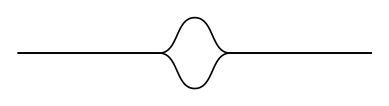
\includegraphics[width=0.10\textwidth]{p147_d1.png}}.
\end{equation}
既然我们只是在做拓扑，就可以稍微松一口气，把它看成圆周上的 $G$-局部系统：
\begin{equation}\tag{10.83}
\Loc_G\!\left(\begin{array}{c}G\\[1pt] \text{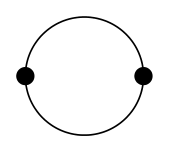
\includegraphics[width=0.05\textwidth]{p147_d2.png}}\\[1pt] G\end{array}\right).
\end{equation}
换句话说，我们看的是圆周上的 $G$-理论，而不是区间上带这些特定边界条件的 $G\times G$-理论。

\begin{srcrem}{55}
这个技巧对一般的 Hecke 代数没有类比。
\end{srcrem}

另一种写法如下。我们考虑 Yang--Mills 理论 $\mathcal{Z}_{G\times G}$，并考虑对角边界条件的自界面：
\diageq{10.84}{0.15\textwidth}{p147_d3.png}
现在我们可以想象把体上的 $G\times G$-理论拆成两份，每一份都标以 $G$-理论：
\begin{equation}\tag{10.85}
\text{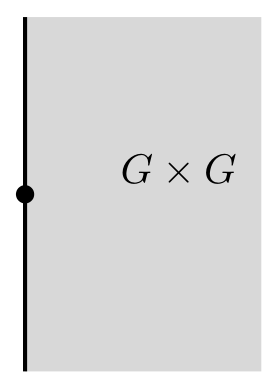
\includegraphics[width=0.10\textwidth]{p148_d1.png}}\;=\;\text{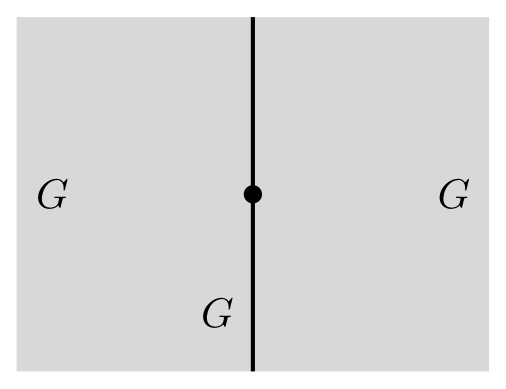
\includegraphics[width=0.17\textwidth]{p148_d2.png}}
\end{equation}
这就是说：$G\times G$-理论的边界条件等同于 $G$-理论的自界面。我们可以把它推广到群的乘积：$G\times H$ 的边界条件等同于 $G$-理论与 $H$-理论之间的界面。

代数上（在足够的对偶性之下），我们这里做的是：
\begin{equation}\tag{10.86}
\Hom(V,W)=V^{*}\otimes W,
\end{equation}
其中左边是界面，右边是乘积理论的边界条件。我们使用的对偶性是 $\C[G]$ 的自对偶性：
\begin{align}
\C[G\times G]\text{-}\mathbf{mod}&=\C[G]\otimes\C[G]\text{-}\mathbf{mod}\tag{10.87}\\
&=\C[G]^{\mathrm{op}}\otimes\C[G]\text{-}\mathbf{mod}\tag{10.88}\\
&=\C[G]\text{-}\mathbf{mod}\text{-}.\tag{10.89}
\end{align}

\begin{srcrem}{56}
这是场论的一个一般事实。一旦理解了边界条件，就理解了界面，反之亦然：场论之间的界面等同于乘积理论的一个边界条件。
\end{srcrem}

\textbf{问题 6.} 为什么 $\mathcal{H}=\mathcal{H}_{G\times G,G}=\C\left[\frac{G}{G}\right]$ 是交换的？

原因是 $\mathcal{H}$ 由 $\mathcal{Z}_G$ 的平凡自界面组成，而后者构成 $\End\big(\mathrm{id}_{\Rep(G)}\big)$。这是 $\Rep(G)$ 的\term{Bernstein 中心}{Bernstein center}。对任意范畴 $\mathcal{C}$，Bernstein 中心是
\begin{equation}\tag{10.90}
\mathcal{Z}(\mathcal{C}):=\End(\mathrm{id}_{\mathcal{C}}).
\end{equation}
断言是：它总是交换的，因为我有两个“方向”来复合这些算子。也就是说，$\mathcal{Z}(\mathcal{C})=\End(\mathrm{id})$ 带有两个相容的幺半结构。一方面，我们可以沿恒等界面碰撞两个界面。另一方面，我们可以把恒等界面的两份自身碰撞，得到：
\begin{equation}\tag{10.91}
\mathrm{id}\circ\mathrm{id}=\mathrm{id}.
\end{equation}
第二种复合对一般的 Hecke 代数没有类比。

\textbf{练习 2.} 带有两个相容幺半结构的集合是交换幺半群。

这是拓扑中 Eckmann--Hilton 论证的玩具版本，后者证明 $\pi_2(X)$ 是交换的。

% [Tutor Note: (10.89) 原文写作“$=\C[G]\text{-}\mathrm{mod}\text{-}$”，末尾的短横线表示右侧还有一个作用未写出，完整写法应为 $\C[G]\text{-}\mathrm{mod}\text{-}\C[G]$（即 $\C[G]$-双模）；这是原文的省略式写法。真正关键的一步是 $\C[G\times G]=\C[G]\otimes\C[G]$ 与 $\C[G]\simeq\C[G]^{\mathrm{op}}$（$g\mapsto g^{-1}$）给出 (10.87)--(10.89) 的链，从而把“乘积理论”翻译成“界面”。]

\begin{srcex}{58}
若 $\mathcal{C}=A\text{-}\mathbf{mod}$，则
\begin{align}
\mathcal{Z}(\mathcal{C})&=\End(\mathrm{id}_{A\text{-}\mathbf{mod}})\tag{10.92}\\
&=\End({}_A A_A),\tag{10.93}
\end{align}
因为如下函子等价：
\begin{equation}\tag{10.94}
(-)\otimes{}_A A_A=\mathrm{id}_{A\text{-}\mathbf{mod}}.
\end{equation}
我们再一次把体上的 $A\otimes A^{\mathrm{op}}$ 理论（边界上带 $A$）“展开”，得到一个体上为 $A$-理论、带平凡界面的理论。但这正好是代数的中心：
\begin{align}
\mathcal{Z}(\mathcal{C})&=\End({}_A A_A)\tag{10.95}\\
&=\mathrm{Z}(A).\tag{10.96}
\end{align}
\end{srcex}

于是对任意范畴 $\mathcal{C}$，我们有一个交换代数 $\mathcal{Z}(\mathcal{C})$。然后我们可以考虑空间：
\begin{equation}\tag{10.97}
\mathcal{M}_{\mathcal{C}}:=\Spec\mathcal{Z}(\mathcal{C}).
\end{equation}
之后我们应当尝试用 $\mathcal{M}_{\mathcal{C}}$ 上的谱分解来理解 $\mathcal{C}$。

\begin{srcex}{59}
若 $\mathcal{C}=A\text{-}\mathbf{mod}$，则我们在 $\Spec\mathrm{Z}(A)$ 上做谱分解。
\end{srcex}

这可能有趣，也可能没有意思，因为中心可能是平凡的。例如在量子力学中，可观测量代数像 Weyl 代数，其中心平凡，于是我们什么也得不到。但断言是：高维 QFT 具有内在的交换性。想法如下。我们考虑体上的理论 $\mathcal{Z}_G$，带一个平凡界面。这等价于理论 $\mathcal{Z}_G$ 有一个 $0$ 维奇点。而这是一个\emph{局部算子}。所以结论是：这种交换性实际上来自局部算子，而不是来自边界条件。

\subsection{物理学中的局部算子}\label{sec:10-5-3}

\term{局部算子}{local operator}是某种局域在时空中一点附近的可观测量。形式上大概是这样的。想法是：在时空中一点的周围，我们考虑半径为 $\epsilon$ 的球面 $S^{n-1}_{\epsilon}$。然后考虑当 $\epsilon\to0$ 时这个球面上的态，它们组成局部算子。所以这类似于该点的一个小去心邻域上场的泛函。注意我们允许在该点处有奇性。

物理学家会告诉你：给定 $x$ 点处的局部算子 $\mathcal{O}_x$，我们可以取期望值：
\begin{equation}\tag{10.98}
\langle\mathcal{O}_x\rangle=\int_{\mathrm{Fields}}\mathcal{O}_x(\varphi)\,e^{-S(\varphi)}\,D\varphi,
\end{equation}
其中我们在 $M\setminus x$ 上对场 $\varphi$ 积分。更一般地，我们有不同点处算子之间的关联函数：
\begin{equation}\tag{10.99}
\big\langle\mathcal{O}_x\mathcal{O}'_y\mathcal{O}''_z\big\rangle=\int \mathcal{O}_x(\varphi)\,\mathcal{O}_y(\varphi)\,\mathcal{O}''_z(\varphi)\,e^{-S(\varphi)}\,D\varphi.
\end{equation}
物理学家还会告诉你的另一件事是\term{算子乘积展开}{operator product expansion}（OPE）：我们尝试取这些点碰撞的极限。于是若从远处看，这些点看起来彼此很近，处于同一个小球内，因此看起来像一个新的复合算子。

在（共形以及）TFT 中，我们有\term{态—算子对应}{state-operator correspondence}：
\begin{equation}\tag{10.100}
\mathcal{Z}\big(S^{n-1}\big)=\text{局部算子的空间},
\end{equation}
其中我们不再需要担心球面的半径。于是 $M\setminus B_{\epsilon}(x)$（即该点某邻域的补）是一个从 $S^{n-1}$ 到 $\varnothing$ 的配边，它给出期望值：
\begin{equation}\tag{10.101}
\langle-\rangle\colon \mathcal{Z}\big(S^{n-1}\big)\longrightarrow\mathcal{Z}(\varnothing_{n-1})=\C.
\end{equation}
所以我们可以直接把局部算子的空间定义为对余维 $1$ 球面的赋值。

\begin{srcex}{60}
考虑有限群 $G$ 的二维 Yang--Mills 理论 $\mathcal{Z}_G$。则局部算子是：
\begin{equation}\tag{10.102}
\mathcal{Z}_G\big(S^1\big)=\C\left[\frac{G}{G}\right].
\end{equation}
对 $\gamma\in\frac{G}{G}$，我们有 delta 函数 $\delta_{\gamma}\in\C\left[\frac{G}{G}\right]$。设 $\Sigma$ 是闭的拓扑曲面。则 $\Sigma\setminus D_x$（即绕该点的一个圆盘的补）是一个配边 $S^1\to\varnothing$。这给出
\begin{equation}\tag{10.103}
\langle-\rangle\colon\C\left[\frac{G}{G}\right]\longrightarrow\C.
\end{equation}
于是
\begin{equation}\tag{10.104}
\langle\delta_{\gamma}\rangle=\#\Loc_G(\Sigma\setminus D,\gamma)
\end{equation}
是绕 $x$ 有单值 $\gamma$ 的 $G$-局部系统的数目。注意这依赖于所处的 Riemann 曲面。
\end{srcex}

关键点是：$\mathcal{H}_{G\times G,G}$ 正好是 $\mathcal{Z}_G$ 中局部算子的代数，而通过画如下图形：
\begin{equation}\tag{10.105}
\text{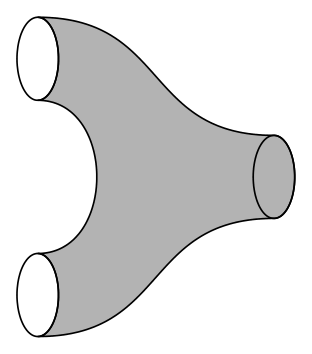
\includegraphics[width=0.12\textwidth]{p150_d1.png}}\;=\;\text{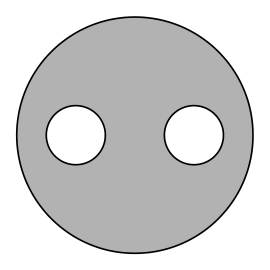
\includegraphics[width=0.11\textwidth]{p150_d2.png}}
\end{equation}
我们得到一个交换的代数结构，因为我们可以让 $x$ 与 $y$ 互相绕行。所以 TFT 中的局部算子（维数 $\ge2$）构成交换代数。

% [Tutor Note: (10.98) 中的积分是形式记号：TFT 中并无真正的测度 $D\varphi$，作者只是借用物理写法来表达“对去心邻域的场求和”。真正严格的表述是 (10.100)--(10.101)：局部算子就是 $\mathcal{Z}(S^{n-1})$，而期望值是从 $S^{n-1}$ 到 $\varnothing$ 的配边所给的线性泛函。另外 (10.104) 的 $\delta_\gamma$ 是共轭类 $\gamma$ 上的 delta 函数，在 $G$ 有限时 $\langle\delta_\gamma\rangle$ 就是一个加权计数，依赖 $\Sigma$ 的拓扑（亏格）。]

\begin{flushright}\small 第 22 讲；2021 年 4 月 15 日\end{flushright}

% ============================================================================
\section{局部算子}\label{sec:10-6}

\begin{sectionkey}
TFT 中的局部算子是 $Z(S^{n-1})$，而把两点处的球面“挤”到一起给出乘法；对 $n\ge2$，$S^{n-1}$ 的链环有足够空间让两点互换，故乘积交换。取谱得到真空模空间，一切东西都成为其上的模——这就是 TFT 的谱分解。
\end{sectionkey}

在\emph{拓扑}场论中，局部算子组成 $\mathcal{Z}\big(S^{n-1}\big)$。

\begin{figure}[htbp]
  \centering
  
\includegraphics[width=0.30\textwidth]{figure10-3.png}
  \caption{挖去两个小 $3$-球之后的 $3$-球。这是从 $S^2\sqcup S^2$ 到 $S^2$ 的配边。（原文 p.~151，Figure 10.3）}
  \label{fig:10-3}
\end{figure}

% [Tutor Note: 原文 Figure 10.4 只有图题、没有图形（p151 留白），疑为原稿遗漏；本译本照译图题而绝不伪造图形。该图本应画出“挖去三个 $3$-球”的情形，用来看乘积的结合性：中间的球面把两个小球隔开，从而两种“先乘哪一对”的顺序给出同一条配边。下文的 (10.108)--(10.110) 正是这一结合性的二维图示版本。]

\begin{figure}[htbp]
  \centering
  \caption{一个挖去三个 $3$-球的 $3$-球。我们可以把其中两个看成位于某个中间球面之内，这就显示了由图~10.3 所定义的乘积的结合性。（原文 p.~151，Figure 10.4；原缺图形）}
  \label{fig:10-4}
\end{figure}

\subsection{代数结构}\label{sec:10-6-1}

考虑 $n$ 维圆盘 $D^n$ 中的两个点。挖去这两个点的小邻域之后，我们得到图~10.3，它是如下配边：
\begin{equation}\tag{10.106}
S^{n-1}\sqcup S^{n-1}\longrightarrow S^{n-1}.
\end{equation}
TFT $\mathcal{Z}$ 把它送到映射：
\begin{equation}\tag{10.107}
\mathcal{Z}\big(S^{n-1}\big)\otimes\mathcal{Z}\big(S^{n-1}\big)\longrightarrow\mathcal{Z}\big(S^{n-1}\big).
\end{equation}
于是我们得到一族局部算子的乘积，由 $D^n$ 中两个球的位置构型来标记。因为 $\mathcal{Z}$ 是拓扑场论，它在“两点位于 $n$-圆盘中”的构型空间上是局部常值的，所以只依赖于该构型空间的 $\pi_0$。那么这个构型空间的 $\pi_0$ 是什么？

若 $n=1$，则我们考虑的是一个区间内两个（各含一点的、小区间的）点。于是有两种情形：$x$ 在 $y$ 之前，或 $y$ 在 $x$ 之前。所以这个空间不连通，也就是说，我们有两个先验不同的乘积：$\mathcal{O}_x*\mathcal{O}'_y$ 与 $\mathcal{O}'_y*\mathcal{O}_x$。于是我们得到一个结合但未必交换的代数。

（原稿批注：fix fig.\ 10.4——此处待补图~10.4。）事实上，我们在任意维数都能得到结合性。要看到这一点，考虑图~10.4。这个配边是图~10.3 的两份的复合。在二维情形，我们从一个较大的圆盘中挖去两个小圆盘，如图~10.5。

\begin{figure}[htbp]
  \centering
  
\includegraphics[width=0.34\textwidth]{figure10-5.png}
  \caption{“马裤”配边。这是从 $S^1\sqcup S^1$ 到 $S^1$ 的配边。（原文 p.~152，Figure 10.5）}
  \label{fig:10-5}
\end{figure}

于是复合对应于：
\diagram[0.16\textwidth]{p152_d3.png}
即 (10.108)（上方第一幅：两个“马裤”沿中间的管复合）、(10.109)（中间一幅：它同伦于一个挖去三个小圆盘的圆盘）与 (10.110)（下方一幅：它又同伦于先右后左的另一种复合），这就证明了结合性。
\begin{equation}\tag{10.108}
\text{两副“马裤”沿中间管道复合}
\end{equation}
\begin{equation}\tag{10.109}
\text{同伦于：一个圆盘挖去三个小圆盘}
\end{equation}
\begin{equation}\tag{10.110}
\text{又同伦于：交换左右顺序后的复合}
\end{equation}
若 $n>1$，则圆盘中一对圆盘（或同伦地，一对点）的构型空间是连通的。这告诉我们：
\begin{equation}\tag{10.111}
\big(\mathcal{Z}(S^{n-1}),\,*\big)
\end{equation}
是一个交换代数。

\begin{srcrem}{57}
这是拓扑量子场论的一个关键特征。量子力学本质上不交换，但一旦进入更高维数，我们就有了这种交换性。
\end{srcrem}

% [Tutor Note: 结合性的两张图不要“从字面上”看混：(10.108) 是“先粘左边一对、再粘第三个”，(10.110) 是“先粘右边一对、再粘第一个”，两者都同伦于 (10.109)（一个圆盘挖去三个小圆盘），所以乘积结合。交换性则是另一回事：它需要两点在构型空间中可以互换，这只有当 $n\ge2$（此时 $\pi_0$ 为单点，甚至 $n\ge3$ 时基本群平凡）才成立。]

\subsection{谱分解}\label{sec:10-6-2}

正如我们已经看到的，一般原则是：如果有人递给你一个交换代数，你就应当取它的 $\Spec$。于是给定 $n$ 维 TFT（$n>1$），我们可以定义一个仿射簇：
\begin{equation}\tag{10.112}
\mathcal{M}_{\mathcal{Z}}^{0}:=\Spec\Big(\mathcal{Z}\big(S^{n-1}\big),\,*\Big).
\end{equation}
这称为\term{真空模空间}{moduli space of vacua}，即这个空间的一点是场论的一个\term{真空}{vacuum}。真空是定义配分函数、期望值等所需数据的一部分。例如，对定义在 $\R^{n}$ 上的量子场论，我们可能尝试定义 $\R^{n}$ 上的配分函数，但由于 $\R^{n}$ 非紧，它不会被良好定义。所以我们需要在无穷远处固定一些数据，也就是在无穷远处紧化；而我们这里看到的是 $\mathcal{Z}\big(S^{n-1}\big)$ 的一个元素。

\begin{srcrem}{58}
我们最初是通过看非常靠近一点的算子（例如在\emph{紫外}）而遇见 $\mathcal{Z}\big(S^{n-1}\big)$ 的。现在我们看到 $\mathcal{Z}\big(S^{n-1}\big)$ 通过看非常远的地方（即在无穷远）而出现。这两者一致，因为\emph{拓扑}量子场论不知道大球面与小球面的区别。换句话说，对拓扑场论，紫外与红外变得相同。在通常的量子场论中，真空与局部算子之间的联系没有这么直接。
\end{srcrem}

给定局部算子 $\mathcal{O}$ 与真空 $\langle0\rangle$，我们可以定义 $\mathcal{O}$ 的真空期望值，即某个数，写作 $\langle0|\mathcal{O}|0\rangle$。所以我们只需把真空看成为使这些期望值有良好定义而需要选择的东西。也就是说，算子给出真空空间上的函数。在 TFT 的框架里，我们将用这一点作为真空的\emph{定义}：真空是 $\Spec\mathcal{Z}\big(S^{n-1}\big)$ 中的一点。

要点是：TFT 同义反复地在其模空间 $\mathcal{M}_{\mathcal{Z}}^{0}$ 上谱分解。也就是说，TFT 中的一切都是 $\mathcal{Z}\big(S^{n-1}\big)$ 上的线性对象。

这是一个代数，所以它当然作用于自身；但周围还有许多其他自然的模。设 $M$ 是 $(n-1)$-流形。那么断言是：$\mathcal{Z}(M)$ 是 $\mathcal{Z}\big(S^{n-1}\big)$ 上的模。考虑配边 $M\times I$，它诱导 $\mathcal{Z}(M)$ 上的恒等映射。然后在区间的某一点处，我们可以认为插入了一个算子，即在该点周围挖去一个小球，得到图~10.6。所得的流形 $(M\times I)\setminus D_x$ 是一个（原稿批注：redo figure——此图待重画）配边：
\begin{equation}\tag{10.113}
M\sqcup S^{n-1}\longrightarrow M,
\end{equation}
它诱导映射：
\begin{equation}\tag{10.114}
\mathrm{act}_x\colon \mathcal{Z}(M)\otimes\mathcal{Z}\big(S^{n-1}\big)\longrightarrow\mathcal{Z}(M).
\end{equation}
这个映射通过画与图~10.4 类似的图把 $\mathcal{Z}(M)$ 实现为模。因此我们可以把 $\mathcal{Z}(M)$ 看成模空间上的层：
\begin{equation}\tag{10.115}
\mathcal{Z}(M)\in \QC\big(\mathcal{M}_{\mathcal{Z}}^{0}\big)=\mathcal{Z}\big(S^{n-1}\big)\text{-}\mathbf{mod}.
\end{equation}

\begin{figure}[htbp]
  \centering
  
\includegraphics[width=0.55\textwidth]{figure10-6.png}
  \caption{从 $M^{n-1}\times I$ 中挖去一个小球，得到从 $M^{n-1}\sqcup S^{n-1}$ 到 $M^{n-1}$ 的配边。这诱导出 $\mathcal{Z}\big(M^{n-1}\big)$ 上的模结构。（原文 p.~154，Figure 10.6）}
  \label{fig:10-6}
\end{figure}

\begin{srcrem}{59}
对每一点 $x\in M$，我们都有 $\mathcal{Z}\big(S^{n-1}\big)$ 在 $\mathcal{Z}(M)$ 上的作用。于是这个巨大的张量积 $\otimes_{x\in M}\mathcal{Z}\big(S^{n-1}\big)$ 作用在 $\mathcal{Z}(M)$ 上，但实际上它通过所谓的\term{因子化同调}{factorization homology}分解：
\begin{equation}\tag{10.116}
\int_{M}\mathcal{Z}\big(S^{n-1}\big),
\end{equation}
它由从 $M$ 到真空模空间的局部常值映射上的函数组成：
\begin{equation}\tag{10.117}
\mathcal{O}\big(\mathrm{Map}_{\mathrm{l.c.}}(M,\mathcal{M}_{\mathcal{Z}})\big).
\end{equation}
\end{srcrem}

% [Tutor Note: (10.112) 的 $\Spec$ 里是交换代数 $(\mathcal{Z}(S^{n-1}),*)$，而不是某个向量空间；$\mathcal{M}_{\mathcal{Z}}^{0}$ 是“真空模空间”，它未必光滑、未必约化。(10.116) 的因子化同调 $\int_M$ 不是普通积分，而是把每一点的局部算子代数沿着 $M$ 装配起来的余极限；当 $M$ 连通时它常退化为 $\mathcal{Z}(S^{n-1})$，这正是 (10.115) 中 $\QC(\mathcal{M}^0_{\mathcal{Z}})=\mathcal{Z}(S^{n-1})\text{-}\mathbf{mod}$ 的来源。]

\subsection{二维 TFT}\label{sec:10-6-3}

局部算子组成态空间 $\mathcal{Z}\big(S^1\big)$。上一次我们研究它时，考虑的是 $\mathcal{Z}$ 与自身之间的恒等界面，然后取 $\End(\mathrm{id}_{\mathcal{C}})$（其中 $\mathcal{C}$ 是边界条件的范畴）。回忆这是 Bernstein 中心
\begin{equation}\tag{10.118}
\End(\mathrm{id}_{\mathcal{C}})=\mathcal{Z}(\mathcal{C}).
\end{equation}
所以这与 $\mathcal{Z}\big(S^1\big)$ 相同。若 $\mathcal{Z}=\mathcal{Z}_G$ 是有限群 $G$ 的二维 Yang--Mills 理论，则
\begin{equation}\tag{10.119}
\mathcal{Z}_G\big(S^1\big)=\C\left[\frac{G}{G}\right]
\end{equation}
（带卷积）是群代数 $\C G$ 的中心。

真空模空间是：
\begin{align}
\mathcal{M}_{\mathcal{Z}_G}^{0}&=\Spec\mathcal{Z}_G\big(S^1\big)\tag{10.120}\\
&=\Spec\C\left[\frac{G}{G}\right]\tag{10.121}\\
&=:\widehat{G},\tag{10.122}
\end{align}
我们将称之为群 $G$ 的\term{酉对偶}{unitary dual}。断言是：$\widehat{G}$ 是 $G$ 的不可约表示的等价类的集合。有限群的表示由 Maschke 定理分解为不可约表示：
\begin{equation}\tag{10.123}
\Rep(G)\simeq\bigoplus_{\text{不可约表示 }V_\lambda\text{ 的等价类}}(\Vect)\otimes V_\lambda.
\end{equation}
也就是说，任何表示可以写成：
\begin{equation}\tag{10.124}
V\simeq\bigoplus_{\lambda\in\widehat{G}}V_\lambda^{\oplus m_\lambda}.
\end{equation}
换言之：
\begin{equation}\tag{10.125}
\Rep(G)\simeq\Vect\big(\widehat{G}\big)=\QC\big(\widehat{G}\big).
\end{equation}
这是谱分解的一个版本。

我们说 $\mathcal{Z}\big(M^{n-1}\big)$ 是 $\mathcal{Z}\big(S^{n-1}\big)$ 上的模。但在二维情形我们得不到太多东西，因为没有多少紧的 $1$-流形。不过我们确实有有意思的带边界的 $1$-流形，例如
\begin{equation}\tag{10.126}
\textcolor{red}{\bullet}\!\!-\!\!-\!\!-\!\!-\!\!\textcolor{blue}{\bullet},
\end{equation}
其中 $V,W\in\Rep(G)$。然后我们有从这个流形到自身、并挖去一个小圆盘的配边：
\diageq{10.127}{0.17\textwidth}{p155_d1.png}
因此 $\mathcal{Z}\big(S^1\big)$ 作用在：
\begin{equation}\tag{10.128}
\mathcal{Z}\big(S^1\big)\curvearrowright
\mathcal{Z}\Big(\textcolor{red}{\bullet}\!\!-\!\!-\!\!-\!\!-\!\!\textcolor{blue}{\bullet}\Big)
=\Hom(V,W)
\end{equation}
也就是说，范畴 $\Rep(G)$ 在 $\mathcal{Z}\big(S^1\big)$-模中富化。等价地，这是一个 $\mathcal{Z}\big(S^1\big)$-线性范畴。

这并不是有限群理论的特例。在任意二维 TFT 中，边界条件的范畴 $\mathcal{C}$ 都是 $\mathcal{Z}\big(S^1\big)=\mathcal{Z}(\mathcal{C})$-线性的。事实上任意范畴 $\mathcal{C}$ 都在 $\mathcal{Z}(\mathcal{C})=\End(\mathrm{id})$ 上线性。这是使 $\mathcal{C}$ 线性的泛代数。也就是说，$\mathcal{C}$ 中的 $\Hom$ 空间自然地落在 $\QC(\Spec\mathcal{Z}(\mathcal{C}))$ 中。想法是：$\mathcal{C}$ 构成 $\mathcal{M}=\Spec\mathcal{Z}(\mathcal{C})$ 上的范畴层。这意味着 $\Hom$ 空间被升级为该空间上的层，即它们是 $\mathcal{Z}(\mathcal{C})$ 上的模。

一般地，我们可以说 $\mathcal{C}$ 是 $R$-线性的，如果 $\Hom$ 空间是 $R$-模，或者等价地，如果存在映射 $R\to\mathcal{Z}(\mathcal{C})$。如果我们处于“大”的设定，即 $\mathcal{C}$ 有足够多的余极限（余完备），那么这等价于说 $\mathcal{C}$ 是 $R\text{-}\mathbf{mod}$ 上的模范畴。

于是我们有三个不同的想法，我们希望把它们内化为同一件事：
\begin{enumerate}
\item $\mathcal{C}$ 构成（拟凝聚的）范畴层；
\item $\mathcal{C}$ 是 $R$-线性的，即存在映射 $R\to\mathcal{Z}(\mathcal{C})$；
\item $\mathcal{C}$ 是 $R\text{-}\mathbf{mod}$ 上的模范畴。
\end{enumerate}
也就是说：$\mathcal{C}$ 是 $\Spec R$ 上的（拟凝聚）范畴层，等价于存在映射 $R\to\mathcal{Z}(\mathcal{C})$，等价于 $\mathcal{C}$ 在 $R$-模中富化，这又说明 $\mathcal{C}$ 带有 $(\mathbf{mod}\text{-}R,\otimes_R)$ 的作用。最后这个刻画看起来有点不同。为了对 $M\in R\text{-}\mathbf{mod}$ 与 $C\in\mathcal{C}$ 定义 $M\otimes C$ 之类的东西，我们先把 $M$ 消解为自由模的复形：
\begin{equation}\tag{10.129}
\cdots\longrightarrow R^{\oplus n_2}\longrightarrow R^{\oplus n_1}\longrightarrow M,
\end{equation}
其中映射是元素在 $R$ 中的矩阵。我们知道 $\mathcal{C}$ 与自由模 $R^{\oplus n_1}$ 的张量积就是 $\mathcal{C}^{\oplus n_1}$。由于范畴是 $R$-线性的，我们可以把这些同样的矩阵写成如下对象之间的映射：
\begin{equation}\tag{10.130}
\cdots\longrightarrow \mathcal{C}^{\oplus n_2}\longrightarrow \mathcal{C}^{\oplus n_1},
\end{equation}
而这是 $M\otimes C$ 的一个消解。这里正是我们用到余极限假设的地方：我们需要写下这些消解并在最后取其余极限。例如群/结合代数的模满足这一点。

\paragraph{局部化}

若 $\mathcal{C}$ 是 $R\text{-}\mathbf{mod}$ 上的模，我们可以在 $\Spec R$ 上定义它的局部化。回忆对通常的模，我们把 $M$ 关于 $R$ 的局部化定义为：
\begin{equation}\tag{10.131}
\underline{M}(U)=M\otimes_R\mathcal{O}(U),
\end{equation}
其中 $U\subset\Spec R$ 是开集。要点是：$\mathcal{O}(U)=R[S^{-1}]$（对某个乘性子集 $S$），于是 $\underline{M}(U)=M[S^{-1}]$。这给出 $R\text{-}\mathbf{mod}$ 与 $\Spec R$ 上拟凝聚层之间的范畴等价。

在范畴的设定下同样的图像也适用。设 $\mathcal{C}\curvearrowright R\text{-}\mathbf{mod}$，于是我们可以构造：
\begin{equation}\tag{10.132}
\underline{\mathcal{C}}(U)=\mathcal{C}\otimes_{R\text{-}\mathbf{mod}}R[S^{-1}]\text{-}\mathbf{mod},
\end{equation}
其中 $U=\Spec R[S^{-1}]$。这就是把 $\mathcal{C}$ 中所有来自 $S\subset R$ 的态射求逆所得的范畴。

对结合代数 $A$（例如 $\C G$），$A\text{-}\mathbf{mod}$ 在 $\Spec\mathcal{Z}(A)$ 上成层。类似地，$\Rep(G)$ 在 $\widehat{G}$ 上成层；而我们可以把表示分解为不可约表示这一事实给出：
\begin{equation}\tag{10.133}
\Rep(G)\simeq\QC\big(\widehat{G}\big).
\end{equation}
这听起来像某种 Fourier 变换的版本，但它并不是典范的。这幅图像里有点可疑之处。同义反复地为真的事情是：$\Rep(G)$ 在中心上成层。给定 $\widehat{G}$ 的任意子集 $S$，我们可以构造 $\Rep(G)$ 的一个直和项，由所有特征落在 $S$ 中的表示组成。但为了得到 $\Rep(G)$ 与 $\Vect^{\widehat{G}}$ 之间的等同，我们需要选取同构类的代表元。另一种办法是，Wedderburn 定理（有限群的 Peter--Weyl 定理）告诉我们：
\begin{equation}\tag{10.134}
\C G\simeq\bigoplus_{V_\lambda\ \text{不可约}}\End(V_\lambda),
\end{equation}
其中 $\End(V_\lambda)=M_{n_\lambda\times n_\lambda}(\C)$，而 $n_\lambda=\dim V_\lambda$。也就是说，$\C G$ 分解为 $\widehat{G}$ 上若干个结合代数的直和，而这些结合代数原来是除代数上的矩阵代数。

这可不是小问题。如果记录“实性”，即考虑实表示，这个同构就不再成立。于是我们考虑 $G$ 的实表示，并看不可约特征的集合 $\widehat{G}$，它带有自然的实结构。不可约表示 $V$ 有三种类型。Schur 引理告诉我们，我们得到 $\R$ 的某个扩域上的除代数：
\begin{equation}\tag{10.135}
\End(V)=\begin{cases}\R\\ \C\\ \HH\end{cases}.
\end{equation}
$\R$ 与 $\HH$ 对应于对偶的实点：$\widehat{G}_{\R}$。复的情形意味着对偶中有复共轭成对的点，即特征不是实值的。但即使特征实值，$\End(V)$ 也不一定是 $\R$，而只是 $\R$ 上的某个除代数。这告诉我们：Wedderburn 分解并不给出 $V$ 的自同态，我们得到的是这个四元数版本。于是 $\QC\big(\widehat{G}\big)$ 作为可逆模范畴非平凡地作用在 $\Rep_{\R}(G)$ 上。也就是说，$\Rep_{\R}(G)$ 是一个范畴化的线丛（$\QC\big(\widehat{G}\big)$ 的可逆模），即一个\term{Gerbe}{Gerbe}。这些对应于 Brauer 群的元素（例如四元数 $\HH$ 在 $\R$ 的 Brauer 群中）。这个 gerbe 与物理学中所谓的\term{反常}{anomaly}有关。

同义反复地为真的是：$\mathcal{C}$ 在 $\mathcal{M}$ 上成层。最简单的答案就是它恰为 $\QC(\mathcal{M})$ 本身。下一个最复杂的情形是 gerbe（$\QC$ 的反常或扭转版本），或者还可能更复杂。

对二维 TFT $\mathcal{Z}$，我们附上局部算子的交换环 $\mathcal{Z}\big(S^1\big)$，它是 $\mathcal{Z}$ 中可观测量代数的一个版本；我们通过用这些算子作用来做观测。于是我们发现 $\mathcal{Z}$ 在 $\mathcal{M}_{\mathcal{Z}}$ 上成层。

\begin{srcrem}{60}
Mednykh 公式告诉我们：
\begin{align}
\mathcal{Z}_G\big(\Sigma^{g}\big)&=\#\Loc_G\Sigma^{g}\tag{10.136}\\
&=\sum_{\chi\in\widehat{G}}\left(\frac{|G|}{\dim(V_\chi)}\right)^{2g-2}.\tag{10.137}
\end{align}
\end{srcrem}

\begin{flushright}\small（原稿批注：transition。）\end{flushright}

\begin{flushright}\small 第 23 讲；2021 年 4 月 20 日\end{flushright}

到目前为止我们已经看到：
\begin{itemize}
\item $\mathcal{Z}\big(S^{n-1}\big)$（局部算子的空间）对 $n\ge2$ 构成交换环；
\item $\mathcal{Z}\big(M^{n-1}\big)$ 自然地是 $\mathcal{Z}\big(S^{n-1}\big)$ 上的模；
\item $\mathcal{Z}\big(N^{n-2}\big)$ 自然地在 $\mathcal{Z}\big(S^{n-1}\big)$ 上线性。
\end{itemize}
我们只对二维 TFT 看到了最后一点，但它在一般情形也成立。要看到这一点，考虑从 $N^{n-2}\times I$ 到自身的恒等配边，即 $(N^{n-2}\times I)\times I$。然后我们挖去一个小圆盘，得到如下配边：
\diageq{10.138}{0.17\textwidth}{p157_d2.png}
这里我们把那个点看成 $N^{n-2}$，也就是说，我们暗中把整幅图与 $N^{n-2}$ 作乘积。于是我们有
\begin{equation}\tag{10.139}
\mathcal{Z}\big(\textcolor{red}{\bullet}\!\!-\!\!-\!\!-\!\!\textcolor{blue}{\bullet}\big),
\end{equation}
它是 $\mathcal{Z}\big(N^{n-2}\big)$ 中的一个 $\Hom$-空间，实际上是交换环 $\mathcal{Z}\big(S^{n-1}\big)$ 上的模。

然后我们发现，可以用如下簇来组织这个结构：
\begin{equation}\tag{10.140}
\mathcal{M}_{\mathcal{Z}}^{\mathrm{aff}}=\mathcal{M}_{\mathcal{Z}}^{0}:=\Spec\mathcal{Z}\big(S^{n-1}\big),
\end{equation}
称为真空模空间。想法是：我们可以把任意的理论 $\mathcal{Z}$ 与一个拉格朗日场论联系起来，后者的场空间是映入 $\mathcal{M}_{\mathcal{Z}}^{0}$ 的映射空间。这些就是我们将在下一节定义的 B-模型。

\begin{srcex}{61}
若 $\mathcal{Z}_G$ 是有限群 $G$ 的二维 Yang--Mills 理论，则 $\mathcal{M}_{\mathcal{Z}}^{0}=\widehat{G}$，这就给出 $\mathcal{Z}$ 分解为不可约部分。
\end{srcex}

% [Tutor Note: (10.136) 左边原文印作 $\mathcal{Z}_G(\Sigma^{G})$，上标是大写 $G$，按意义应为亏格 $g$（右边写的是 $\Sigma^{g}$ 与 $2g-2$），这是原稿的笔误，照译并指出。另外“$\Rep(G)$ 在 $\widehat{G}$ 上成层”并不是典范的：如作者所述，要把它变成真正的 $\QC(\widehat{G})$，需要选代表元；实表示的情形只能得到 gerbe，这正是物理上“反常”的几何来源。]

% ============================================================================
\section{B-模型}\label{sec:10-7}

\begin{sectionkey}
对任意交换环 $R$，用“局部常值映射”构造截断的 B-模型：$(n-1)$-流形给函数环、$(n-2)$-流形给模范畴，推拉由对应给出。于是任一 TFT 都能与它的谱上的 B-模型比较，谱分解就是说“理论是高一维 B-模型的边界条件”。
\end{sectionkey}

设 $R$ 是交换环（等价地，可以想成簇 $X=\Spec R$）。由它我们可以构造任意维数的（截断）TFT。这里“截断”的意思是：我们不去关心给最高维配边附上数。这是一个拉格朗日场论，所以对流形 $M$ 我们有场的概念，由下式给出：
\begin{equation}\tag{10.141}
\mathrm{Map}(M,\Spec R=X).
\end{equation}
我们如何让光滑流形与仿射簇之间产生有趣的相互作用？我们将考虑它们之间能考虑的“最笨”的相互作用：局部常值映射。也就是说，我们考虑：
\begin{equation}\tag{10.142}
\mathrm{Map}_{\mathrm{lc}}(M,X)=\mathrm{Map}(\pi_0(M),X).
\end{equation}
用环的语言，这就是：
\begin{equation}\tag{10.143}
\mathrm{Map}_{\mathrm{lc}}(M,X)=\Spec\big(R\otimes\pi_0(M)\big).
\end{equation}
然后我们可以如下定义 $X=\Spec R$ 上的（截断）$n$ 维 B-模型。对 $(n-1)$-流形我们赋予：
\begin{equation}\tag{10.144}
B_X^{n}\big(M^{n-1}\big)=\mathcal{O}\big(\mathrm{Map}(M,X)\big)=R\otimes\pi_0(M).
\end{equation}
对 $(n-2)$-流形我们赋予：
\begin{equation}\tag{10.145}
B_X^{n}\big(N^{n-2}\big)=\QC\big(\mathrm{Map}(N,X)\big)=\big(R\otimes\pi_0(N)\big)\text{-}\mathbf{mod}.
\end{equation}
然后可以由如下对应（span，即双拉回图）定义你想要的任何推拉运算：
\begin{equation}\tag{10.146}
\begin{array}{ccc}
& \mathrm{Map}(M,X) &\\[4pt]
\swarrow & & \searrow\\[4pt]
\mathrm{Map}(\partial_{\mathrm{in}},X) & & \mathrm{Map}(\partial_{\mathrm{out}},X)
\end{array}
\end{equation}

这与谱分解有什么关系？我们从一个 $n$ 维 TFT $\mathcal{Z}$ 出发，然后构造了这个环 $\big(\mathcal{Z}(S^{n-1}),*\big)$，并由它定义 B-模型
\begin{equation}\tag{10.147}
B_{\mathcal{M}_{\mathcal{Z}}^{0}}^{n}.
\end{equation}
朴素的想法是：$\mathcal{Z}$ 看起来像理论 $B_{\mathcal{M}_{\mathcal{Z}}^{0}}^{n}$。

\begin{srcex}{62}
考虑有限群 $G$ 的二维 Yang--Mills 理论 $\mathcal{Z}_G$。则 $\mathcal{M}_{\mathcal{Z}}^{0}=\widehat{G}$，
\begin{equation}\tag{10.148}
\mathcal{Z}_G\big(S^1\big)=\C\left[\frac{G}{G}\right]\simeq\C\big[\widehat{G}\big]
\end{equation}
是局部算子的环，而
\begin{equation}\tag{10.149}
\mathcal{Z}_G(\mathrm{pt})=\Rep(G)\simeq\QC\big(\widehat{G}\big),
\end{equation}
它也是 $B_{\mathcal{M}_{\mathcal{Z}}^{0}}^{2}(\mathrm{pt})$。也就是说，我们只看这个类函数环就能重建理论。
\end{srcex}

\begin{srcrem}{61}
镜像对称正是这类想法。事实上，Gross--Siebert 的“内蕴镜像对称”就是紧密仿照这个想法构造的。从一个有意思的理论出发（原稿批注：cite——此处需补文献），即引用辛拓扑中的 A-模型；然后构造一个簇（镜像），作为局部算子环的谱。接着镜像对称说：你出发时的 A-模型与你所构造的 B-模型是等价的。
\end{srcrem}

即使对有限群 $G$，$\Rep_{\R}G$ 也不会恰好等于朴素的答案 $\QC\big(\widehat{G}\big)$。

相反，靠抽象废话，我们得到如下结果。我们知道 $\mathcal{Z}\big(M^{n-1}\big)$ 是 $\mathcal{Z}\big(S^{n-1}\big)$ 上的模。我们通过与区间作乘积并插入一个局部算子而得到这个结构，也就是如图~10.6 那样挖去一个小球。所以实际上，对 $M$ 中每一点我们都得到一个模结构族，使得当我们沿两点之间的路径走时，相应的作用被等同起来。也就是说，它局部常值地依赖于 $x\in M$。于是我们自然得到：$\mathcal{Z}(M)$ 是 $\mathcal{Z}\big(S^{n-1}\big)$ 的 $\pi_0(M)$ 多份拷贝上的模，即如下作用：
\begin{equation}\tag{10.150}
\pi_0(M)\otimes\mathcal{Z}\big(S^{n-1}\big)=\mathcal{O}\big(\mathrm{Map}(M,\mathcal{M}_{\mathcal{Z}}^{0})\big).
\end{equation}
所以我们并没有得到这个向量空间与这个环之间的同构，而是得到：$\mathcal{Z}(M)$ 是 $\mathcal{O}\big(\mathrm{Map}(M,\mathcal{M}_{\mathcal{Z}}^{0})\big)$ 上的模，即它是一个对象：
\begin{equation}\tag{10.151}
\mathcal{Z}(M)\in \QC\big(\mathcal{M}_{\mathcal{Z}}^{0}\big),
\end{equation}
也就是说
\begin{equation}\tag{10.152}
\mathcal{Z}(M)\in B_{\mathcal{M}_{\mathcal{Z}}^{0}}^{n+1}(M).
\end{equation}
同样，$\mathcal{Z}(N)$ 是 $R$-线性范畴，但实际上它可以细化为一个在 $\pi_0(N)\otimes R$ 上线性的范畴，即
\begin{equation}\tag{10.153}
\mathcal{Z}(N)\in B_{\mathcal{M}_{\mathcal{Z}}^{0}}^{n+1}(N)=\text{$\mathcal{M}_{\mathcal{Z}}^{0}$ 上的范畴层 $2$-范畴}.
\end{equation}

总结一下：场论的谱分解是这样说的。我们从 $n$ 维 TFT $\mathcal{Z}$（即我们的态）出发。然后我们有可观测对象（局部算子），它们作用在态上。我们可以把它重新表述为：
\begin{equation}\tag{10.154}
\mathcal{Z}(-)\in B_{\mathcal{M}_{\mathcal{Z}}^{0}}^{n+1}(-).
\end{equation}
等价地说，理论 $\mathcal{Z}$ 是这个高一维的 B-模 $B_{\mathcal{M}_{\mathcal{Z}}^{0}}^{n+1}$ 的边界条件。也就是说，我们把 $M\times I$ 带一个红色（标以 $\mathcal{Z}$ 的）边界：
\diageq{10.155}{0.15\textwidth}{p159_d2.png}
我们最初把边界条件想成群表示，或一般地，想成范畴的对象。我们这里所做的只是同一想法的更精致版本。

回忆我们当时正走向这些四维 A-模型。我们只讨论了群 $G=\mathrm{GL}_1$ 的情形，其中我们得到拓扑 Maxwell 理论 $\mathcal{A}_{\mathrm{GL}_1}$。这个理论赋予三维流形 $M^3$ 的向量空间 $\mathcal{A}_{\mathrm{GL}_1}(M^3)$，是 $\mathrm{Pic}(M^3)$ 上的局部常值函数。回忆 $\mathrm{Pic}(M^3)$ 是 $U(1)$-联络模规范等价的空间。现在我们可以问局部算子是什么，并尝试像上面那样玩谱分解的游戏。

回忆 $\mathrm{Pic}(M)$ 看起来像格 $H^2(M,\Z)$ 与一个环面的交叉，后者有 $\pi_1=H^1(M,\Z)$。局部算子将来自对 $S^3$ 的赋值，但 $S^3$ 既没有 $H^2$ 也没有 $H^1$，所以我们得到
\begin{equation}\tag{10.156}
\mathrm{Pic}\big(S^3\big)=\mathrm{pt}.
\end{equation}
如果我们对自同构小心一点，这里可能得到 $BU(1)$ 之类的东西。无论如何，其上的局部常值函数是平凡的，所以我们没有任何局部算子。在导出版本中我们会得到：
\begin{equation}\tag{10.157}
H^{*}\big(BU(1)\big)=\C[u],
\end{equation}
但这仍然不太有意思/有用。

% [Tutor Note: 本节要抓住“比较”的逻辑：任给交换环 $R$ 都有截断 B-模型 $B^n_X$（局部常值映射），它是“最简单的拉格朗日理论”；对任意 TFT $\mathcal{Z}$，用它的局部算子环造出 $B^{n+1}_{\mathcal{M}^0_{\mathcal{Z}}}$，谱分解的准确内容就是 (10.152)--(10.154)：$\mathcal{Z}$ 是该 B-模型的边界条件，而不是说 $\mathcal{Z}$ 与它相等。$R\otimes\pi_0(M)$ 是“每个连通分支一份 $R$”的简写，不要理解成真的张量积。]

% ============================================================================
\section{缺陷}\label{sec:10-8}

\begin{sectionkey}
把“标记点”换成“嵌入子流形”，局部算子的故事就推广为缺陷：余维 $k$ 缺陷由 $Z(S^{k-1})$ 标记。线算子（$k=2$）随维数升高依次得到 $E_1$、$E_2$、$E_\infty$ 结构；四维时线算子的谱给出 $\mathcal{M}^1_Z$，它是 $\mathcal{M}^0_Z$ 的仿射化。
\end{sectionkey}

现在我们要把关于局部算子的故事推广到线算子。为此我们将引入一般的缺陷算子，而这又需要讨论配边假设。

\subsection{配边假设}\label{sec:10-8-1}

（原稿批注：fix and cite——此处需补文献。）配边假设由 Baez--Dolan 提出，并由 Hopkins--Lurie、Lurie、Ayala--Francis、Schommer--Pries 证明。配边假设是拓扑场论中的某些概念与范畴论中的某些概念之间的等价。我们将把它看成从范畴数据构造拓扑场论的方法。也可以反过来看，即把它看成对“为什么各种图示演算能描述范畴论”的解释：它告诉我们，可以画图而不必去想范畴。

\term{扩展拓扑场论}{extended topological field theory}是配边范畴的一个表示，即一个对称幺半函子：
\begin{equation}\tag{10.158}
\mathcal{Z}\colon\big(\Bord_n^{\square},\sqcup\big)\longrightarrow\big(\mathcal{C},\otimes\big),
\end{equation}
其中 $\square$ 可以是任意选定的\term{切向结构}{tangential structure}。例如，我们可能要求配边是定向的、标架的，或一般地具有 $G$-结构（只要有一个映射 $G\to O(n)$）。若 $G=1$，则 $G$-结构就是 $n$-标架。若 $G=SO(n)$，则 $G$-结构等价于在 $M$ 上选取一个定向。若 $G=O(n)$，则 $M$ 上的 $G$-结构不包含任何额外结构。无论如何，要画的基本图像是：这个范畴中的流形总带有 $n$ 维切丛。也就是说，与一个点不同，我们可以画一小块 $\R^n$。

配边假设说：场论 $\mathcal{Z}$ 的结构完全由数据 $\mathcal{Z}(\mathrm{pt})\in\mathcal{C}$ 决定，但要服从：
\begin{itemize}
\item 可对偶性（有限性条件）；
\item 自对偶结构（这依赖于 $\square$）。
\end{itemize}
对一维理论，可对偶性问的是赋予点的向量空间是否有对偶。自对偶约束与切向结构的选择有关。

\subsection{带奇点的配边假设}\label{sec:10-8-2}

（原稿批注：Cite——此处需补文献。）这出现在 Lurie 的工作中，是 Baez--Dolan 的一个猜想（称为\emph{tangle 猜想}）的推广。我们把配边假设描述为拓扑场论与范畴论之间的某种等价。到目前为止，配边假设的陈述只告诉我们对象层面的等价，并没有反映我们在范畴论中看到的某些图示结构，例如态射、高阶态射、自同态等等——而这些在带奇点的配边假设的帮助下会变得更明显。一般的想法是：我们现在描述的是定义在更大源上的场论，即定义在带某些指定奇点的配边上的场论，而这些奇点将与某些范畴结构相匹配。

\begin{figure}[htbp]
  \centering
  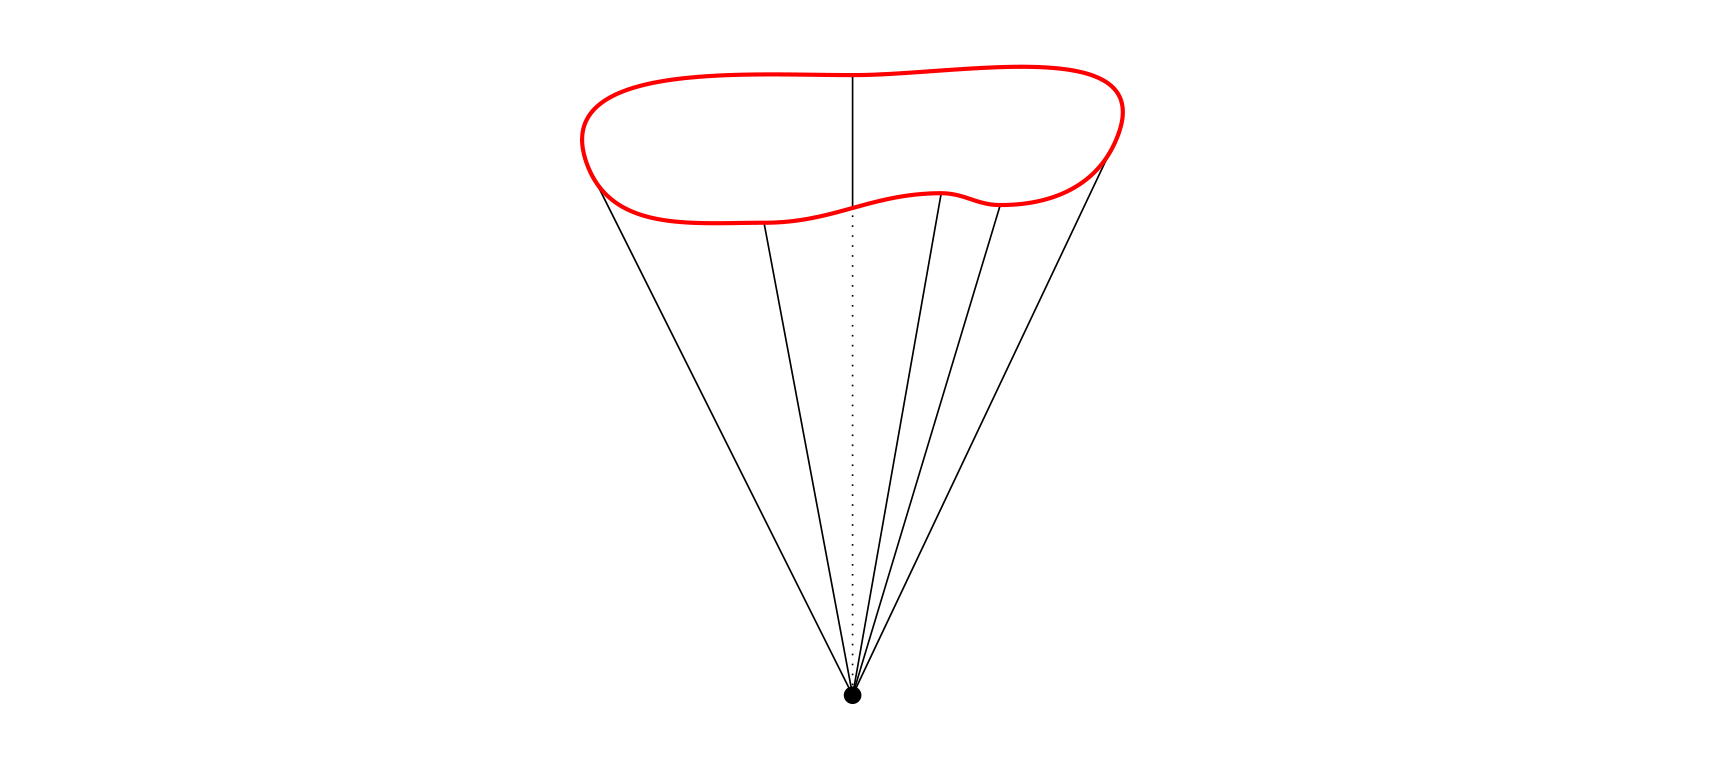
\includegraphics[width=0.42\textwidth]{figure10-7.png}
  \caption{流形 $M$ 的锥：先把 $M$ 与一个区间作乘积，然后把一端上整个 $M$ 的拷贝商掉。原来的流形用红色标出。（原文 p.~161，Figure 10.7）}
  \label{fig:10-7}
\end{figure}

给定流形 $M$，我们可以通过构造 $M$ 上的\term{锥}{cone}来造出奇点，其定义为：
\begin{equation}\tag{10.159}
C(M):=(M\times I)\big/(M\times\{0\}),
\end{equation}
如图~10.7。奇异点周围的链环是 $M$。我们想加入同样风味的奇点。例如，我们可能允许链环由某个流形给出的奇点，或者做某种分层版本，用这样的锥归纳地构造。

带奇点的配边假设粗略地说：从带可能的 $C(M)$-奇点的 $\Bord_n$ 到 $(\mathcal{C},\otimes)$ 的对称幺半函子，等价于：
\begin{enumerate}
\item $\mathcal{Z}\colon\Bord_n\to\mathcal{C}$（或等价地，一个对象 $C\in\mathcal{C}$），连同
\item $\mathcal{Z}(M)$ 的一个对象，即一个态射：
\begin{equation}\tag{10.160}
1\longrightarrow\mathcal{Z}(M).
\end{equation}
\end{enumerate}
想法是：$M$ 上的锥是一条从 $\varnothing$ 到 $M$ 的新配边，$\mathcal{Z}$ 把它送到映射 $1\to\mathcal{Z}(M)$，即 $\mathcal{Z}(M)$ 的一个元素。我们唯一需要的情形是 $M$ 为球面。当我们取以球面为模型的锥时，这其实并不是真正的奇点，但我们仍然可以想象：在构造以球面为模型的锥时指定了一个标记点。例如，如果我们看带标记点的 $\Bord_n$，那么带奇点的配边假设说这个标记点等价于指定一个对象 $\mathcal{O}\in\mathcal{Z}\big(S^{n-1}\big)$，而这是一个局部算子。所以这就是我们已经看到的东西。如果你愿意，这就是局部算子的态—场对应。

这告诉我们：如果我们看 $n$-流形连同嵌入的 $(k-1)$-流形，那么我们需要看奇点的链环（即嵌入子流形），它是一个球面 $S^{n-k}$。所以我们需要给出 $\mathcal{Z}\big(S^{n-k}\big)$ 的一个元素。这些被称为\term{缺陷算子}{defect operator}。例如，线缺陷/线算子是嵌入的 $1$-流形，它们对应于一个态的选择
\begin{equation}\tag{10.161}
L\in\mathcal{Z}\big(S^{n-2}\big).
\end{equation}
所以以前局部算子是向量空间 $\mathcal{Z}\big(S^{n-1}\big)$ 的元素，而现在赋值 $\mathcal{Z}\big(S^{n-2}\big)$ 是线算子的范畴。同样地，$\mathcal{Z}\big(S^{n-3}\big)$ 是曲面缺陷的 $2$-范畴。

要点是：给定 $n$ 维 TFT $\mathcal{Z}$，一旦我们指定了一个元素 $L\in\mathcal{Z}\big(S^{n-2}\big)$（满足适当的可对偶性条件），我们就可以把理论延拓到带任意嵌入 $1$-流形的流形上。也就是说，对任意纽结 $K\subset M$，我们得到新的值：
\begin{equation}\tag{10.162}
\mathcal{Z}_L(M\supset K).
\end{equation}

\begin{srcex}{63}
若 $n=3$，这就是说：我们需要指定一个元素 $L\in\mathcal{Z}\big(S^{n-2}\big)$ 来确定一个纽结不变量。
\end{srcex}

我们看到 $\mathcal{Z}\big(S^{n-1}\big)$ 构成交换环（$n\ge2$），然后取 $\Spec$：
\begin{equation}\tag{10.163}
\mathcal{M}_{\mathcal{Z}}^{0}=\Spec\mathcal{Z}\big(S^{n-1}\big),
\end{equation}
并在其上谱分解，即把态研究成局部算子上的模。

现在我们要对线算子玩同样的游戏。所以考虑线算子的范畴 $\mathcal{Z}\big(S^{n-2}\big)$。事实上，正如局部算子的向量空间构成代数那样，它也构成一个张量范畴。这个乘积仍然来自所谓的 OPE，但现在是线算子的 OPE 而不是局部算子的。乘积来自图~10.3 中的配边，只不过现在我们把它看成生活在四维空间中，即球面是 $n$ 维空间中绕两条嵌入线的链环 $S^{n-2}$（而不是 $n$ 维空间中绕两个点的链环 $S^{n-1}$）。

换句话说，得到这个结构所需的数据是（更大的）圆盘内部点（或圆盘）的构型。这与我们为局部算子画过的图是同一幅，只是我们现在忽略了更多的维数，所以范畴的层级跳了一级。也就是说，$\mathcal{Z}\big(S^{n-2}\big)$ 带有由“大圆盘内一对圆盘”的构型（局部常值地）标记的乘法。（这意味着它定义在小 $(n-1)$-圆盘算子之上，后者也称为 $E_{n-1}$-结构。）

\begin{srcex}{64}
例如，二维的线算子是余维 $1$ 的，于是我们有由区间内的区间标记的乘法。所以乘法是结合的但不交换。这是一个 $E_1$-结构。
\end{srcex}

\begin{srcex}{65}
在三维中我们有“马裤”：
\diageq{10.164}{0.13\textwidth}{p163_d1.png}
它是从 $S^1\sqcup S^1$ 到 $S^1$ 的配边，因此告诉我们 $\mathcal{Z}\big(S^1\big)$ 有一个运算 $*$，它局部常值地依赖于圆盘内两点的构型空间。更精确地说，我们是指：给定构型之间的一条路径，我们就得到相应乘法之间的一个同构。也就是说，我们得到从基本群胚出发的映射：
\begin{equation}\tag{10.165}
\pi_{\le1}\big(\mathrm{Conf}_2 D^2\big)\otimes\mathcal{Z}\big(S^1\big)^{\otimes2}\longrightarrow\mathcal{Z}\big(S^1\big).
\end{equation}
\end{srcex}
圆盘中两点对的这个空间是连通的，所以在局部算子层面这个乘法是交换的。现在这只说明我们有一个同构 $L_1*L_2\simeq L_2*L_1$，但当我们把它平方时，并不能保证得到恒等：
\begin{equation}\tag{10.166}
L_1*L_2\xrightarrow{\ \sim\ }L_2*L_1\xrightarrow{\ \sim\ }L_1*L_2
\qquad\big(\text{复合是否为 }\mathrm{id}?\big)
\end{equation}
于是我们发现：$\mathcal{Z}\big(S^1\big)$ 仍是幺半的，但现在它甚至是\term{辫状幺半}{braided monoidal}的，即这个乘法运算满足辫关系。我们可以想象圆盘中多个点的构型通过一个辫变成另一个构型：
\diageq{10.167}{0.16\textwidth}{p163_d3.png}
这给出一个同构：
\begin{equation}\tag{10.168}
L_1*L_2*L_3\longrightarrow L_3*L_2*L_1,
\end{equation}
而辫关系说这些同构满足辫群的关系。

所以在二维，线算子是 $E_1$，即一个幺半范畴。在三维，线算子是 $E_2$，即一个辫状幺半范畴。但在四维及以上，线算子是 $E_\infty$，即对称幺半的。于是基本群胚是：
\begin{equation}\tag{10.169}
\pi_{\le1}\big(\mathrm{Conf}_2 D^{\ge3}\big)=0,
\end{equation}
所以我们平方得到恒等：
\begin{equation}\tag{10.170}
L_1*L_2\xrightarrow{\ \sim\ }L_2*L_1\xrightarrow{\ \sim\ }L_1*L_2
\qquad\big(\text{复合 }=\mathrm{id}\big).
\end{equation}
也就是说，这些空间不只是连通的，事实上还是\emph{单连通}的。

% [Tutor Note: (10.163) 原文写的是 $\mathcal{M}^0_{\mathcal{Z}}=\Spec\mathcal{Z}(S^{m-1})$，上标 $m$ 与上下文（$n$ 维理论）不符，应为 $S^{n-1}$，这是原稿的笔误。(10.166) 与 (10.170) 的区别正是 $\pi_1$ 的作用：$D^2$ 中两点构型空间的基本群是 $\Z$（绕数），所以交换两次只给出辫关系而不保证恒等；而在 $\ge3$ 维，构型空间单连通，平方才是恒等，于是得到对称幺半 $E_\infty$。]

现在我们可以陈述结论了。在四维及以上，线算子：
\begin{equation}\tag{10.171}
\big(\mathcal{Z}\big(S^2\big),*\big)
\end{equation}
构成张量范畴，于是我们可以定义：
\begin{equation}\tag{10.172}
\mathcal{M}_{\mathcal{Z}}^{1}:=\Spec\Big(\mathcal{Z}\big(S^2\big),*\Big).
\end{equation}
这是 $\mathcal{M}_{\mathcal{Z}}^{0}$ 的一个加细。具体地说，它由仿射化给出：
\begin{equation}\tag{10.173}
\mathcal{M}_{\mathcal{Z}}^{1}\twoheadrightarrow\mathcal{M}_{\mathcal{Z}}^{0},
\qquad \mathcal{M}_{\mathcal{Z}}^{0}=\mathrm{Aff}\big(\mathcal{M}_{\mathcal{Z}}^{1}\big).
\end{equation}

% [Tutor Note: (10.171) 原文本应是一个范畴 $\big(\mathcal{Z}(S^2),*\big)$，而 (10.172) 才是对它的谱；这里把“取谱”的对象与谱本身分开写更清楚。$\mathcal{M}^1_{\mathcal{Z}}\to\mathcal{M}^0_{\mathcal{Z}}$ 是仿射化，一般不是同构：线算子比局部算子知道严格更多的信息（见 Remark 64）。]

\begin{flushright}\small（原稿批注：transition。）\end{flushright}

\begin{flushright}\small 第 24 讲；2021 年 4 月 22 日\end{flushright}

% ============================================================================
\subsection{局部算子与线算子}\label{sec:10-8-3}

\begin{sectionkey}
缺陷就是“流形上的标记子流形”，其余维为 $k$ 时由 $Z(S^{k-1})$ 标记。四维时线算子（余维 2）构成张量范畴，其谱 $\mathcal{M}^1_Z$ 是 $\mathcal{M}^0_Z$ 的仿射化；因此线算子严格比局部算子知道得更多。
\end{sectionkey}

回忆 TFT 中的缺陷算子是我们的 TFT 在各维球面上的值：
\begin{itemize}
\item $\mathcal{Z}\big(S^{n-1}\big)$ 由局部算子组成；
\item $\mathcal{Z}\big(S^{n-2}\big)$ 由线算子组成；
\item $\mathcal{Z}\big(S^{n-3}\big)$ 由曲面算子组成，等等。
\end{itemize}
当 $n$（理论的维数）足够大而缺陷的维数足够小时，缺陷构成交换代数。也就是说，一旦球面有足够的空间互相绕行，“碰撞”得到的乘积就变成交换的。例如我们看到，对 $n=1$ 局部算子只是结合的；但对 $n>1$ 它们是交换的。类似地，线算子在 $n=2$ 时结合，$n=3$ 时辫状，$n\ge4$ 时对称。

我们主要关心四维 TFT 中的线算子。它们构成对称幺半范畴 $\big(\mathcal{Z}\big(S^2\big),*\big)$，于是我们取谱：
\begin{equation}\tag{10.174}
\mathcal{M}_{\mathcal{Z}}^{1}:=\Spec\Big(\mathcal{Z}\big(S^2\big),*\Big).
\end{equation}
回忆局部算子 $\mathcal{Z}\big(S^{n-1=3}\big)$ 构成交换代数，所以我们也可以对它取谱，得到：
\begin{equation}\tag{10.175}
\mathcal{M}_{\mathcal{Z}}^{0}=\Spec\mathcal{Z}\big(S^{n-1}\big).
\end{equation}

\textbf{问题 7.} $\mathcal{M}_{\mathcal{Z}}^{1}$ 与 $\mathcal{M}_{\mathcal{Z}}^{0}$ 之间的关系是什么？也就是说，线算子与局部算子之间的关系是什么？

看这个关系的一种方式是用下面这幅漫画。考虑一个局部算子，即大片的“空无一物”中间的一个蓝色小点：
\diageq{10.176}{0.12\textwidth}{p164_d2.png}

我们可以把它解释为：它其实坐在一条透明的、画成红色的线上：
\diageq{10.177}{0.12\textwidth}{p165_d1.png}
也就是说，我们把局部算子看成坐在一条\emph{平凡}的 $1$ 维缺陷上。这个平凡缺陷是线算子上卷积结构的单位。也就是说，\textbf{局部算子等同于平凡线算子的自界面}。

\paragraph{悬垂}

结果表明，这幅图像可以用“对球面作悬垂”来重新表述。假设我们在研究 $S^{n-2}$，它作为一条线的链环出现。那么线算子 $\mathcal{Z}\big(S^{n-2}\big)$ 有一个 特殊的对象：
\begin{equation}\tag{10.178}
\mathcal{Z}\big(D^{n-1}\big)\in\mathcal{Z}\big(S^{n-2}\big),
\end{equation}
因为我们可以把圆盘看成一个配边：
\diageq{10.179}{0.21\textwidth}{p165_d2.png}
即从 $S^{n-2}\to\varnothing$ 的配边。

断言是：这个 特殊的对象就是单位。回忆我们的乘法来自“马裤”配边：
\diageq{10.180}{0.12\textwidth}{p165_d3.png}
于是用圆盘作乘法就是恒等，因为一旦把“马裤”与圆盘复合起来，我们就得到：
\begin{equation}\tag{10.181}
\text{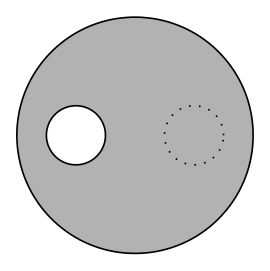
\includegraphics[width=0.10\textwidth]{p165_d4.png}}\;\simeq\;
\text{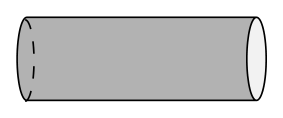
\includegraphics[width=0.10\textwidth]{p165_d5.png}}\;\simeq\;S^{n-2}\times I,
\end{equation}
而这是恒等配边。

我们也可以把圆盘与自身复合，形成一个球面：
\begin{equation}\tag{10.182}
\text{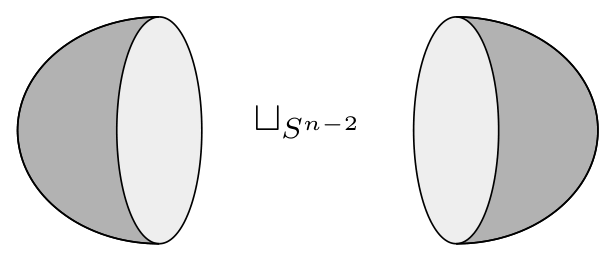
\includegraphics[width=0.15\textwidth]{p166_d1.png}}\;=\;
\text{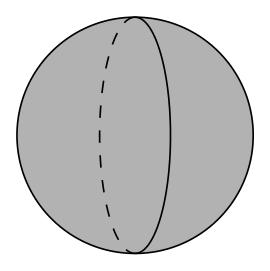
\includegraphics[width=0.09\textwidth]{p166_d2.png}}\;=\;S^{n-1}.
\end{equation}
这恰好就是把 $S^{n-2}$ 悬垂得到 $S^{n-1}$ 的过程。要点是：这幅图给出
\begin{equation}\tag{10.183}
\mathcal{Z}\big(S^{n-1}\big)=\Hom_{\mathcal{Z}(S^{n-2})}\Big(\mathcal{Z}\big(D^{n-1}\big),\mathcal{Z}\big(D^{n-1}\big)\Big)
=\End_{\mathcal{Z}(S^{n-2})}(1).
\end{equation}
也就是说，$\mathcal{Z}\big(S^{n-1}\big)$ 是 $\mathcal{Z}\big(S^{n-2}\big)$ 中单位的自同态。

\begin{srcrem}{62}
如果我们更小心地处理标架等等，圆盘的两份复合起来给出的是\emph{意大利饺}（ravioli）/UFO：
\begin{equation}\tag{10.184}
\text{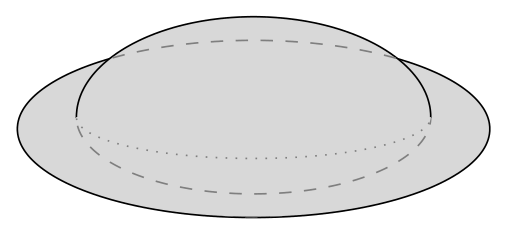
\includegraphics[width=0.15\textwidth]{p166_d3.png}}\;=\;
D^{n-1}\sqcup_{D^{n-1}\backslash\mathrm{pt}}D^{n-1}\;=\;
\text{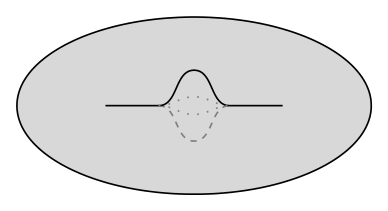
\includegraphics[width=0.12\textwidth]{p166_d4.png}}.
\end{equation}
\end{srcrem}

结论是：局部算子 $\mathcal{Z}\big(S^{n-1}\big)$ 被等同于：
\begin{equation}\tag{10.185}
\mathcal{Z}\big(S^{n-1}\big)=\End\big(1_{\mathcal{Z}(S^{n-2})}\big)=\End(\text{平凡线算子}).
\end{equation}

\begin{srcrem}{63}
这与 \S10.4.3、例~58、\S10.6.3、\S10.7（例~62）中的做法是同一招；在那里我们说：
\begin{equation}\tag{10.186}
\mathcal{Z}_G\big(S^1\big)=\C\left[\frac{G}{G}\right]=\End({}_G\C_G G),
\end{equation}
并把它中的 ${}_G\C_G G$ 解释为 $\mathcal{Z}_G$ 的平凡线缺陷。
\end{srcrem}

这对任意球面都是一般构造。例如，线算子由平凡曲面算子的自同态给出。

\paragraph{仿射化}

于是我们通过 TFT 看到了局部算子与线算子之间的关系，但现在我们想从谱的角度来看它。回忆我们有 $\mathcal{M}_{\mathcal{Z}}^{0}=\Spec\mathcal{Z}\big(S^{n-1}\big)$ 与 $\mathcal{M}_{\mathcal{Z}}^{1}=\Spec\mathcal{Z}\big(S^{n-2}\big)$。我们刚刚看到的是：$\mathcal{Z}\big(S^{n-1}\big)$ 由 $\mathcal{Z}\big(S^{n-2}\big)$ 中单位/平凡对象（即 $\big(\mathcal{M}_{\mathcal{Z}}^{1},\otimes\big)$）的自同态给出。我们知道 $\QC\big(\mathcal{M}_{\mathcal{Z}}^{1},\otimes\big)$ 中的单位是结构层：
\begin{equation}\tag{10.187}
\mathcal{O}_{\mathcal{M}_{\mathcal{Z}}^{1}}\in\QC\big(\mathcal{M}_{\mathcal{Z}}^{1},\otimes\big),
\end{equation}
所以这就是说：
\begin{align}
\mathcal{Z}\big(S^{n-1}\big)&=\mathcal{O}\big(\mathcal{M}_{\mathcal{Z}}^{0}\big)\tag{10.188}\\
&=\End_{\QC(\mathcal{M}_{\mathcal{Z}}^{1})}\big(\mathcal{O}_{\mathcal{M}_{\mathcal{Z}}^{1}}\big)\tag{10.189}\\
&=\Hom\big(\mathcal{O}_{\mathcal{M}_{\mathcal{Z}}^{1}},\mathcal{O}_{\mathcal{M}_{\mathcal{Z}}^{1}}\big)\tag{10.190}\\
&=\Gamma\big(\mathcal{O}_{\mathcal{M}_{\mathcal{Z}}^{1}}\big),\tag{10.191}
\end{align}
因为从 $\mathcal{O}$ 到任何东西的 $\Hom$ 就是那个东西的整体截面。也就是说
\begin{equation}\tag{10.192}
\mathcal{M}_{\mathcal{Z}}^{0}=\Spec\Gamma\big(\mathcal{O}_{\mathcal{M}_{\mathcal{Z}}^{1}}\big)=:\mathrm{Aff}\big(\mathcal{M}_{\mathcal{Z}}^{1}\big),
\end{equation}
因为这就是仿射化的定义。这是代数几何中的一般构造：
\begin{equation}\tag{10.193}
X\longrightarrow\mathrm{Aff}(X):=\Spec\big(\mathcal{O}(X)\big),
\end{equation}
它在如下意义下是泛的：从 $X$ 到仿射簇的任何映射都经过到 $\mathrm{Aff}(X)$ 的映射分解。也就是说，给定一个概形（或栈），我们可以考虑其上的函数；这并不能知道关于它的一切（即大多数对象不是仿射的），但我们仍可以对它取 $\Spec$ 得到仿射化：一个“逼近”原概形的仿射对象。

于是我们有
\begin{equation}\tag{10.194}
\mathcal{M}_{\mathcal{Z}}^{1}\twoheadrightarrow\mathcal{M}_{\mathcal{Z}}^{0}
\end{equation}
是仿射化，即 $\mathcal{M}_{\mathcal{Z}}^{1}$ 是 $\mathcal{M}_{\mathcal{Z}}^{0}$ 的一个新的、改进的版本；也就是说，一般地，线算子严格知道得比局部算子多。

\begin{srcrem}{64}
仿射化可能丢掉大量信息。例如，射影空间 $\PP^{n}$ 的仿射化是一个点，而像 $BG$ 这样的栈的仿射化也是一个点。要点是：代数栈的世界远不止函数环。
\end{srcrem}

于是我们看到：取单位自同态这一范畴论操作，对应于悬垂这一拓扑操作，又对应于相应模空间的仿射化这一代数几何操作。

\begin{srcrem}{65}
我们还可以进一步构造与曲面算子相联系的某个对象 $\mathcal{M}_{\mathcal{Z}}^{2}$：
\begin{equation}\tag{10.195}
\cdots\longrightarrow\mathcal{M}_{\mathcal{Z}}^{2}\longrightarrow\mathcal{M}_{\mathcal{Z}}^{1}\longrightarrow\mathcal{M}_{\mathcal{Z}}^{0}.
\end{equation}
我们不需要这些更高的版本，但 $\mathcal{M}_{\mathcal{Z}}^{1}$ 的构造对我们非常有用。
\end{srcrem}

% [Tutor Note: (10.183)--(10.186) 的核心等式链是 $\mathcal{Z}(S^{n-1})=\End_{\mathcal{Z}(S^{n-2})}(1)$：局部算子是线算子范畴中单位的自同态。这就解释了为什么“局部算子环 = 线算子范畴的中心”。取 $\Spec$ 之后，$1\mapsto\mathcal{O}$（结构层），$\End(\mathcal{O})=\Gamma(\mathcal{O})$ 是整体截面，于是 $\mathcal{M}^0_{\mathcal{Z}}=\Spec\Gamma(\mathcal{O}_{\mathcal{M}^1_{\mathcal{Z}}})$ 恰是仿射化。(10.186) 中 ${}_G\C_G G$ 是双模记号（群的左、右作用）。]

从一个四维 TFT 我们构造了栈 $\mathcal{M}_{\mathcal{Z}}^{1}$，即 TFT $\mathcal{Z}$ 的谱。这对于下面的事情很有用。想法是：这给出我们用所谓 B-模型（\S10.7 引入的简单拉格朗日 TFT）所作的逼近以及与它们的关系。也就是说，我们可以问：$\mathcal{Z}$ 与“映入其模空间/谱 $\mathcal{M}_{\mathcal{Z}}^{1}$ 的映射理论”有多接近？设 $X$ 是簇或栈。回忆对任意 $n$，我们可以构造 $n$ 维截断 TFT，称为 B-模型 $B_X^{n}$，它把 $(n-1)$-流形送到：
\begin{equation}\tag{10.196}
B_X^{n}\big(M^{n-1}\big)=\mathcal{O}\big(\mathrm{Map}_{\mathrm{lc}}(M,X)\big),
\end{equation}
其中映射（场）是局部常值的。对 $X$ 是栈的情形，我们可以做一些比简单构造
\begin{equation}\tag{10.197}
\mathrm{Map}_{\mathrm{lc}}(M,X)=\mathrm{Map}(\pi_0M,X)
\end{equation}
更有意思的事（这是 $X$ 只是簇时我们做的）。回忆栈是函子 $\mathrm{Ring}\to\mathrm{Grpd}$。对 $M$ 为流形，我们可以构造基本群胚
\begin{equation}\tag{10.198}
\pi_{\le1}M,
\end{equation}
其对象是点，态射是模同伦的路径。于是现在我们可以把局部常值映射解释为：
\begin{equation}\tag{10.199}
\mathrm{Map}_{\mathrm{lc}}(M,X)=\mathrm{Map}(\pi_{\le1}M,X).
\end{equation}
要点是：任何流形 $M$ 给出一个函子 $\mathrm{Ring}\to\mathrm{Grpd}$，它就是常函子
\begin{equation}\tag{10.200}
R\mapsto\pi_{\le1}(M).
\end{equation}
因此我们可以把流形与栈看成生活在
\begin{equation}\tag{10.201}
\mathrm{Functors}(\mathrm{Ring},\mathrm{Grpd})
\end{equation}
中。现在我们可以在函子的这个公共范畴中计算 $\mathrm{Map}_{\mathrm{lc}}(M,X)$。其结果是：这些映射记住了 $M$ 的基本群胚，而不仅仅是 $\pi_0$。

\begin{srcex}{66}
设 $X=\mathrm{pt}/G$，$G$ 有限。则
\begin{equation}\tag{10.202}
\mathrm{Map}_{\mathrm{slc}}(M,\mathrm{pt}/G)=\Loc_G M.
\end{equation}
于是 $X$ 的 B-模型由把这个空间 $\mathrm{Map}_{\mathrm{lc}}(M,X)$ 线性化给出：
\begin{align}
B_X^{n}\big(M^{n-1}\big)&=\mathcal{O}\big(\mathrm{Map}_{\mathrm{lc}}(M,X)\big)\tag{10.203}\\
B_X^{n}\big(N^{n-2}\big)&=\QC\big(\mathrm{Map}_{\mathrm{lc}}(N,X)\big)\tag{10.204}\\
B_X^{n}\big(P^{n-3}\big)&=\mathrm{ShvCat}\big(\mathrm{Map}_{\mathrm{lc}}(P,X)\big).\tag{10.205}
\end{align}
\end{srcex}

\paragraph{故事的寓意}

于是我们从 $n$ 维 TFT $\mathcal{Z}$ 出发，构造了谱 $\mathcal{M}_{\mathcal{Z}}^{1}$。由它可以构造两样东西：$B_{\mathcal{M}_{\mathcal{Z}}^{1}}^{n}$ 或 $B_{\mathcal{M}_{\mathcal{Z}}^{1}}^{n+1}$。于是 $\mathcal{Z}$ 在代数几何中最好的逼近是 $B_{\mathcal{M}_{\mathcal{Z}}^{1}}^{n}$。更好的认识是：$\mathcal{Z}$ 在 $\mathcal{M}_{\mathcal{Z}}^{1}$ 上线性，即 $\mathcal{Z}$ 是 $B_{\mathcal{M}_{\mathcal{Z}}^{1}}^{n+1}$ 的边界。

回忆 $\mathcal{Z}\big(N^{n-2}\big)$ 被 $\mathcal{Z}\big(S^{n-2}\big)$ 作用，于是我们发现：对 $N^{n-2}$ 的每一点，$\mathcal{Z}\big(N^{n-2}\big)$ 都有 $\mathcal{Z}\big(S^{n-2}\big)$ 上的模结构。也就是说，不做任何选择，我们就得到 $\mathcal{Z}\big(S^{n-2}\big)$ 的 $\pi_0(N)$ 多份拷贝的一个作用。但实际上我们可以把 $\pi_0$ 换成 $\pi_{\ge1}$。所以之前我们有的是：若两点之间存在通路，则相应的作用同构。现在我们有的是：对它们之间的每条路径都有一个作用之间的同构。也就是说，模结构关于 $x\in N$ 局部常值，于是我们实际上有“从 $N$ 到模空间的局部常值映射”的 $\QC$ 的作用：
\begin{equation}\tag{10.206}
\mathcal{Z}\big(N^{n-2}\big)\curvearrowright\QC\big(\mathrm{Map}_{\mathrm{lc}}(N,\mathcal{M}_{\mathcal{Z}}^{1})\big).
\end{equation}
也就是说，我们有一个范畴 $\mathcal{Z}\big(N^{n-2}\big)$，还有另一个范畴
\begin{equation}\tag{10.207}
B_{\mathcal{M}_{\mathcal{Z}}^{1}}^{n}(N)=\QC\big(\mathrm{Map}_{\mathrm{slc}}(N,\mathcal{M}_{\mathcal{Z}}^{1})\big),
\end{equation}
而前者是后者的模。即 $\mathcal{Z}\big(N^{n-2}\big)$ 是 $B_{\mathcal{M}_{\mathcal{Z}}^{1}}^{n}(N)$ 的一个对象，后者是 $\mathcal{M}_{\mathcal{Z}}^{1}$ 上的范畴层。

\begin{srcrem}{66}
这是把所有这些线算子装配成作用于 $\mathcal{Z}\big(N^{n-2}\big)$ 的对象的一般方式。这个过程称为\term{因子化同调}{factorization homology}。常用如下记号：
\begin{align}
\int_M R&=\mathcal{O}\big(\mathrm{Map}_{\mathrm{lc}}(M,\Spec(R))\big),\tag{10.208}\\
\int_M (\mathcal{C},\otimes)&=\QC\big(\mathrm{Map}_{\mathrm{slc}}(M,\Spec(\mathcal{C}))\big),\tag{10.209}
\end{align}
后者是范畴的情形。
\end{srcrem}

现在我们将看到 $\mathrm{Map}_{\mathrm{slc}}(N,\mathcal{M}_{\mathcal{Z}}^{1})$ 具有恰当类型的结构。对一点 $x\in N$ 我们得到求值映射：
\begin{equation}\tag{10.210}
\begin{array}{c}
\mathrm{Map}_{\mathrm{lc}}(N,\mathcal{M}_{\mathcal{Z}}^{1})\\[2pt]
\downarrow{\scriptstyle \mathrm{ev}_x}\\[2pt]
\mathcal{M}_{\mathcal{Z}}^{1}
\end{array}
\end{equation}
于是我们得到拉回映射：
\begin{equation}\tag{10.211}
\mathrm{ev}_x^{*}\colon \QC\big(\mathcal{M}_{\mathcal{Z}}^{1}\big)\longrightarrow\QC\big(\mathrm{Map}_{\mathrm{lc}}(N,\mathcal{M}_{\mathcal{Z}}^{1})\big).
\end{equation}
所以如果我们有 $\QC\big(\mathrm{Map}_{\mathrm{lc}}(N,\mathcal{M}_{\mathcal{Z}}^{1})\big)$ 在 $\mathcal{Z}\big(N^{n-2}\big)$ 上的作用，我们也得到 $\QC\big(\mathcal{M}_{\mathcal{Z}}^{1}\big)$ 的作用：
\begin{equation}\tag{10.212}
\mathrm{ev}_x^{*}\colon \QC\big(\mathcal{M}_{\mathcal{Z}}^{2}\big)=\mathcal{Z}\big(S^{n-2}\big)\longrightarrow
\QC\big(\mathrm{Map}_{\mathrm{lc}}(N,\mathcal{M}_{\mathcal{Z}}^{2})\big)\curvearrowright\mathcal{Z}\big(N^{n-2}\big).
\end{equation}

\begin{srcrem}{67}
这个图表告诉我们这个操作的局部—整体相容性。也就是说：我们从与点 $x\in N$ 相联系的这些作用出发，它们装配在一起给出更大空间 $\QC\big(\mathrm{Map}_{\mathrm{lc}}(N,\mathcal{M}_{\mathcal{Z}}^{1})\big)$ 的一个作用，然后这些求值映射再把局部的作用取回来。
\end{srcrem}

局部—整体部分要证明的一般定理是：带有对每个 $x\in N$（局部常值地依赖于 $x$）的 $(\mathcal{C},\otimes)$ 的作用的范畴，等价于带有如下作用的范畴：
\begin{equation}\tag{10.213}
\mathcal{C}^{\otimes N}:=\int_N\mathcal{C}:=\QC\big(\mathrm{Map}_{\mathrm{slc}}(N,\Spec\mathcal{C})\big),
\end{equation}
其中 $\mathcal{C}$ 是 Tannakian 的（$\mathcal{C}=\QC(\Spec\mathcal{C})$）。

所以结论是：任意 $n$ 维 TFT $\mathcal{Z}$ 都是 $B_{\mathcal{M}_{\mathcal{Z}}^{1}}^{n+1}$ 的边界条件，即 $\mathcal{Z}(N)$ 在 $\mathrm{Map}_{\mathrm{lc}}(N,\mathcal{M}_{\mathcal{Z}}^{1})$ 上成层。

% [Tutor Note: (10.212) 中的 $\mathcal{M}^2_{\mathcal{Z}}$ 疑为 $\mathcal{M}^1_{\mathcal{Z}}$ 的笔误：这一段的语境全是线算子的谱 $\mathcal{M}^1_{\mathcal{Z}}$ 与 $\mathcal{Z}(S^{n-2})$，而 $\mathcal{M}^2_{\mathcal{Z}}$ 直到 Remark 65 才作为曲面算子的对象正式定义、且并未再使用。照译并指出。另注意 $\mathrm{Map}_{\mathrm{lc}}$ 与 $\mathrm{Map}_{\mathrm{slc}}$（带基本群胚的局部常值映射）的区别正是 (10.199) 与 (10.202) 的差别。]

% ============================================================================
\subsection{回到拓扑 Maxwell 理论}\label{sec:10-8-4}

\begin{sectionkey}
用上一节的抽象机器处理 4 维拓扑 Maxwell 理论 $\mathcal{A}_{\mathrm{GL}_1}$：其线算子是 $\Z$-分次向量空间，谱是 $\mathrm{pt}/\mathbb{G}_m$，于是电侧 $\QC(\Loc_1\Sigma)$ 作用在磁侧 $\mathcal{A}(\Sigma)$ 上。Fourier 变换把这个作用说成“$\mathcal{A}(\Sigma)$ 是 $\mathcal{B}(\Sigma)$ 上的秩 $1$ 自由模”。
\end{sectionkey}

回忆（来自 \S4.5、\S4.8.1、\S6.1.1 与 \S6.4）我们有一个 TFT $\mathcal{A}_{\mathrm{GL}_1}$，它把三维流形送到 $\mathrm{Pic}(M)$ 上的局部常值函数空间。对 Riemann 曲面我们有几个不同的版本。Betti 版本是：
\begin{equation}\tag{10.214}
\mathcal{A}_{\mathrm{GL}_1}\big(\Sigma^2\big)=\Loc\big(\mathrm{Pic}\,\Sigma\big),
\end{equation}
而在 de Rham 版本中我们有：
\begin{equation}\tag{10.215}
\mathcal{A}_{\mathrm{GL}_1}\big(\Sigma^2\big)=\mathbf{D}\text{-}\mathbf{Mod}\big(\mathrm{Pic}\,\Sigma\big).
\end{equation}
回忆这两个范畴并不相同，但非常相似。对于我们眼下要做的事，选哪一个都无所谓。

于是，靠上述抽象废话，对每一点 $x\in\Sigma^2$ 我们都得到 $\mathcal{A}(S^2)$（线算子）在 $\mathcal{A}(\Sigma^2)$ 上的作用。对 $S^2=\Sigma$ 我们选取一个复结构，于是可以把它想成 $\PP^1$，并且有
\begin{equation}\tag{10.216}
\mathcal{A}\big(S^1\big)=\Loc\big(\mathrm{Pic}(\PP^1)\big)=\Loc(\Z)=\Vect^{\Z\text{-gr}},
\end{equation}
其中复合积就是分次向量空间的张量积，即由 $\Z$ 上的群结构诱导的乘积。我们可以把这理解为：当我们有时……

\begin{srcrem}{68}
复合积由整数加法诱导，这一事实是 Gauss 定律的一个版本。这个复合积由配边 $\PP^1\sqcup\PP^1\to\PP^1$ 诱导（即从一个 $3$-球内部挖去两点）。我们可以想象在这两点处各有一个磁单极子，整数值被解释为它们的磁通量；然后当我们看得更远——即进入大的/目标 $\PP^1$ 内部——时，磁通量相加。
\end{srcrem}

也就是说，我们的线算子（'t Hooft/Dirac 线算子）对应于 $\Z$-分次向量空间。这告诉我们：我们的模空间由对 $\Vect^{\Z\text{-gr}}$ 作 Tannakian 重构给出。回忆例~37 中我们有：
\begin{equation}\tag{10.217}
\mathcal{M}_{\mathcal{A}_{\mathrm{GL}_1}}=\Spec\big(\Vect^{\Z\text{-gr}}\big)=\mathrm{pt}/\mathbb{G}_m.
\end{equation}
因此：
\begin{align}
\mathrm{Map}_{\mathrm{lc}}\big(\Sigma,\mathcal{M}_{\mathcal{A}}^{1}\big)&=\mathrm{Map}_{\mathrm{lc}}\big(\Sigma,\mathrm{pt}/\mathbb{G}_m\big)\tag{10.218}\\
&=\Loc_1(\Sigma).\tag{10.219}
\end{align}
所以我们发现 $\mathcal{A}(\Sigma^2)$ 被 $\QC(\Loc_1\Sigma)$ 作用，而回忆（来自 \S6.4.2）这正是 B-侧赋予曲面 $\Sigma$ 的东西：
\begin{equation}\tag{10.220}
\QC\big(\Loc_1\Sigma\big)=\mathcal{B}(\Sigma).
\end{equation}
于是我们发现：磁理论 $\mathcal{A}(\Sigma)$ 被电理论 $\mathcal{B}(\Sigma)$ 作用。但这并不是我们所说的。我们说过它们等价。于是我们接下来要说明的是：$\mathcal{A}(\Sigma)$ 是一个秩 $1$ 自由模，因此一旦选定一个生成元，它就同构于 $\mathcal{B}(\Sigma)$；也就是说，我们只需跟踪单位。

\begin{srcrem}{69}
我们讲了一阵子电磁对偶，把它说成涉及交换群论的 Fourier 变换。我们在这里发现的是：你并不真的需要那套交换群论。只从场论 $\mathcal{A}$ 出发，谱/电侧就是我们能内在地从 $\mathcal{A}$ 构造出来的东西。
\end{srcrem}

所以结论是：自守侧是
\begin{equation}\tag{10.221}
\mathcal{A}_G\big(\Sigma^2\big)=\Shv\big(\Bun_G(\Sigma)\big),
\end{equation}
（其中 $\mathcal{A}_G$ 是参数 $\Psi=0$ 的 GL-扭转 $\mathcal{N}=4$ 超 Yang--Mills 理论），然后由它我们构造某种谱侧 $\QC(-)$，后者作用在 $\mathcal{A}_G(\Sigma)$ 上。几何 Langlands 猜想说这两者是相同/密切相关的。

% [Tutor Note: (10.216) 左边原文印作 $\mathcal{A}(S^1)$，但线算子的链环在四维中是 $S^2$，且本段讨论的是 $S^2=\Sigma\cong\PP^1$ 上的线算子，故这里应为 $\mathcal{A}(S^2)$，是原稿的指标笔误。链路上：$\mathrm{Pic}(\PP^1)=\Z$ 是离散空间，其上的局部系统 (= $\Loc(\Z)$) 就是 $\Z$-分次向量空间，这正是 (10.216) 右边写成 $\Vect^{\Z\text{-gr}}$ 的原因；而 $\QC(\Loc_1\Sigma)$ 与 $\Loc(\mathrm{Pic}\,\Sigma)$ 是同一个范畴的两种描述（Tannakian / Fourier 对偶），这是几何 Langlands 中“电—磁”两侧的关键识别。]

\begin{flushright}\small 第 25 讲；2021 年 4 月 22 日\end{flushright}

% ============================================================================
\subsection{拓扑 Maxwell 理论}\label{sec:10-8-5}

\begin{sectionkey}
把对每一点的局部作用装配起来就是因子化同调 $\int_\Sigma R$；对 $\mathcal{A}_{\mathrm{GL}_1}$，这给出 $\QC(\Loc_{\mathbb{G}_m}\Sigma)$ 作用于磁侧。Fourier 变换的现代表述是“自守侧是谱侧的秩 $1$ 自由模”，由此进入几何 Langlands 的 Hecke 对应。
\end{sectionkey}

（原稿批注：transition。）回忆我们有一个四维 TFT $\mathcal{Z}$，对一个拓扑曲面 $\Sigma$，我们看 $\mathcal{Z}(\Sigma)$。它有一个对称代数，即局部算子代数 $\mathcal{Z}\big(S^2\big)$，它作用在 $\mathcal{A}(\Sigma)$ 上。特别地，对每一点 $x\in\Sigma$ 我们都可以挖去一个球：
\begin{equation}\tag{10.222}
x\in\Sigma\times\{i\}\subset\Sigma\times I
\end{equation}
得到一个配边 $\Sigma\sqcup S^2\to\Sigma$，$\mathcal{Z}$ 把它送到作用 $\mathcal{Z}\big(S^2\big)\otimes\mathcal{Z}(\Sigma)\to\mathcal{Z}(\Sigma)$。也就是说，对每一点 $x\in\Sigma$ 我们都得到一个作用。然后给定从 $x$ 到 $y$ 的一条路径，我们得到相应作用的等同；类似地，给定路径之间的路径（以此类推），我们得到等同之间的等同（以此类推）。于是从 TFT 我们得到一个交换代数（在范畴中）的作用，由 $x\in\Sigma$ 标记，关系由路径给出，关系之间的关系由路径之间的路径给出，以此类推。

这就是如下一般构造。给定交换代数 $R$（在任意带某些余极限的对称幺半（高阶）范畴 $(\mathcal{C},\otimes)$ 中）以及拓扑空间 $\Sigma$。那么，把 $\Sigma$ 只看成单纯集，我们可以构造 $R\otimes\Sigma$，它仍是 $\mathcal{C}$ 中的交换代数。简言之，它就是 $R^{\otimes\#\mathrm{vertices}(\Sigma)}$，关系由 $1$-单形给出，以此类推。这称为 $R$ 在 $\Sigma$ 上的\term{因子化同调}{factorization homology}，记作
\begin{equation}\tag{10.223}
\int_\Sigma R=R\otimes\Sigma.
\end{equation}
当交换环 $R$ 足够好（Tannakian）时，它有具体的几何描述：
\begin{equation}\tag{10.224}
R\otimes\Sigma=\mathcal{O}\big(\mathrm{Map}_{\mathrm{lc}}(\Sigma,\Spec(R))\big).
\end{equation}
对好的张量范畴 $R$（而不是交换环），我们有：
\begin{equation}\tag{10.225}
R\otimes\Sigma=\QC\big(\mathrm{Map}_{\mathrm{lc}}(\Sigma,\Spec(R))\big).
\end{equation}
现在我们将用它来研究规范理论。回忆我们处于拓扑 Maxwell 理论 $\mathcal{A}_{\mathrm{GL}_1}$ 的设定中。它没有局部算子，但有有意思的线算子，即余维 $3$ 缺陷。我们在 \S4.5.1 见过这些缺陷。给定三维流形 $M^3$，我们可以在一点处造一个 Dirac 磁单极子，并通过在这个点周围的 $2$-球面上给定某个磁通量，得到向量空间 $\mathcal{A}(M)$ 的一个新版本。同一想法的另一种变体如下。考虑 $M^3$ 并让时间流逝，即考虑 $M^3\times I$；余维 $3$ 的奇点将是 $M^3\times I$ 中的一个圈/纽结。这个奇点的链环将是 $S^2$，而现在我们可以研究这个柱面 $M^3\times I$ 上的丛，它们在 $2$-球面上有某个整的 Chern 类/通量。前一种线算子的表现修改了赋予 $M^3$ 的向量空间，后一种图像则给出 $\mathcal{Z}(M)$ 与自身之间的算子。

我们知道线算子组成 $\mathcal{Z}\big(S^2\big)$，在这个情形中它由下式给出：
\begin{equation}\tag{10.226}
\mathcal{A}_{\mathrm{GL}_1}\big(S^2\big)=\text{$\mathrm{Pic}(S^2)$ 上的层}=\Vect^{\Z\text{-gr}}.
\end{equation}
也就是说，给定三维流形 $M$、一点 $p\in M$ 以及一个 $\Z$-分次向量空间，我们得到赋予 $M$ 的 Hilbert 空间的一个新版本，它是按不同电荷/单极数加权的和。我们还有分次维数：
\begin{equation}\tag{10.227}
\dim_{\mathrm{gr}}\colon \Vect^{\Z\text{-gr}}\longrightarrow\C^{\Z},
\end{equation}
即给定 $\Z$-分次向量空间，我们得到整数的一个复线性组合。回忆我们在 $M\times I$ 中用单极数的复线性组合来标记纽结。所以这些分次向量空间给我们这些线算子，我们可以把它们绕在四维流形中真正的纽结/圈上。
% [Tutor Note: 这里的字典是：$\mathrm{Pic}(S^2)=\Z$ 是离散空间，其上的局部系统就是 $\Z$-分次向量空间，第 $k$ 个分量对应单极数 $k$ 的态；于是线算子范畴 $\mathcal{A}_{\mathrm{GL}_1}(S^2)=\Vect^{\Z\text{-gr}}$。(10.227) 的 $\dim_{\mathrm{gr}}$ 把每个分次维数读成一个整数，这正是把线算子绕在纽结上时按单极数加权的“迹”。[译者按（无外部依据）：由本章 (10.214)、(10.226)--(10.227) 及 Remark 68 的 Gauss 定律讨论推得]]

要点是：在规范理论中，余维 $3$ 缺陷有很大的活动空间。更详细地说：在 $3$ 维及以上我们可以看余维 $3$ 缺陷，其链环是 $2$-球面，而 $S^2$ 上 Yang--Mills 方程的解很有意思。这里我们谈的是交换情形，它只由单极数给出；现在我们将考虑非交换情形。这种一般类型的算子称为 \term{'t Hooft 算子}{'t Hooft operator}。

于是我们有：$\mathcal{A}_{\mathrm{GL}_1}(\Sigma)$ 被 $\Vect^{\Z\text{-gr}}$ 在每一点 $x\in\Sigma$ 处作用。我们可以把这些作用装配成 $\Sigma\otimes\Vect^{\Z\text{-gr}}$ 的作用，它可以写成：
\begin{align}
\Sigma\otimes\Vect^{\Z\text{-gr}}&=\Sigma\otimes\Rep(\mathbb{G}_m)\tag{10.228}\\
&=\Sigma\otimes\QC\big(\mathrm{pt}/\mathbb{G}_m\big)\tag{10.229}\\
&=\QC\big(\mathrm{Map}_{\mathrm{slc}}(\Sigma,\mathrm{pt}/\mathbb{G}_m)\big)\tag{10.230}\\
&=\QC\big(\Loc_{\mathbb{G}_m}(\Sigma)\big).\tag{10.231}
\end{align}
这个范畴正是 B-侧/电侧/谱侧赋予 $\Sigma$ 的东西：
\begin{equation}\tag{10.232}
\mathcal{B}_{\mathrm{GL}_1}(\Sigma):=\Sigma\otimes\mathcal{A}_{\mathrm{GL}_1}\big(S^2\big)=\QC\big(\Loc_{\mathbb{G}_m}(\Sigma)\big).
\end{equation}
所以 B/电/谱侧作用在 A/磁/自守侧上。一旦我们认识到 $\mathcal{A}$ 是 $\mathcal{B}$ 上的秩 $1$ 自由模，这就归结为“这些理论（在 Fourier 变换下）等价”的陈述。

我们可以在 Fourier 变换的层面看到这是如何运作的。我们习惯于 Fourier 变换给出同构：
\begin{equation}\tag{10.233}
\big(\mathrm{Fun}(G),*\big)\simeq\big(\mathrm{Fun}(G^{\vee}),\cdot\big),
\end{equation}
但我们可以把它重新表述为：$\mathrm{Fun}(G)$ 是 $\mathrm{Fun}(G^{\vee},\cdot)$ 上的秩 $1$ 模，带一个 特殊的单位。也就是说，我们有一个作用：
\begin{equation}\tag{10.234}
\big(\mathrm{Fun}(G^{\vee},\cdot)\big)\curvearrowright\mathrm{Fun}(G),
\end{equation}
由与特征作卷积给出。然后我们断言 $\mathrm{Fun}(G^{\vee})$ 事实上是秩 $1$ 自由模。对 $G$ 是群，$\delta_e\in\mathrm{Fun}(G)$ 是单位，所以我们可以作用在 $\delta_e$ 上得到：
\begin{equation}\tag{10.235}
\mathrm{Fun}(G^{\vee})\xrightarrow{\ \sim\ }\mathrm{Fun}(G).
\end{equation}
然后 Fourier 变换说这是同构。所以我们想把观点转变为以这种方式看待 Fourier 变换。

在 Betti 版本中，对 $\Sigma$ 为 Riemann 曲面，我们附上一个范畴：
\begin{equation}\tag{10.236}
\mathcal{A}_{\mathrm{GL}_1}(\Sigma)=\Loc\big(\mathrm{Pic}(\Sigma)\big).
\end{equation}
现在我们需要选一个单位，以便得到与“它作为模所依托的东西”的等同。我们想说的是 $\mathrm{Pic}$ 的单位处的摩天楼层层：$\mathcal{O}\in\mathrm{Pic}$。在 de Rham 版本中我们有 $\mathcal{A}_{\mathrm{GL}_1}(\Sigma)=\mathbf{D}\text{-}\mathbf{Mod}(\mathrm{Pic})$，所以我们可以直接取它。但在 Betti 版本中，这个摩天楼层层实际上并不在 $\Loc(\mathrm{Pic}(\Sigma))$ 中，所以我们需要找一个替代物如下。我们有包含：
\begin{equation}\tag{10.237}
i\colon\{\mathcal{O}\}\hookrightarrow\mathrm{Pic},
\end{equation}
然后我们可以取 $\mathrm{Pic}$ 的万有覆盖（关于基点 $\mathcal{O}$），它给出一个可缩空间 $\widetilde{\mathrm{Pic}}$ 映射到 $\mathrm{Pic}$：
\begin{equation}\tag{10.238}
\begin{array}{ccc}
\{\mathcal{O}\} & \xrightarrow{\ i\ } & \mathrm{Pic}\\[4pt]
& \searrow{\scriptstyle \widetilde{\pi}} & \uparrow{\scriptstyle \widetilde{\pi}}\\[4pt]
& & \widetilde{\mathrm{Pic}}
\end{array}
\end{equation}
% [Tutor Note: 图中 $\{\mathcal{O}\}\to\mathrm{Pic}$ 是包含 $i$；两条标作 $\widetilde{\pi}$ 的箭头分别是基点的提升 $\{\mathcal{O}\}\to\widetilde{\mathrm{Pic}}$ 与覆盖投影 $\widetilde{\mathrm{Pic}}\to\mathrm{Pic}$，二者复合即 $i$。正因为 $\widetilde{\mathrm{Pic}}$ 可缩，常层 $k$ 在它上面就是“平凡数据”，沿 $\widetilde{\pi}$ 前推（(10.239) 的 $\widetilde{\pi}_*(k)$）便得到 $\Loc(\mathrm{Pic})$ 中一个并非有限秩的局部系统——它是 de Rham 版本中单位处摩天楼层层的替身。[译者按（无外部依据）：由本章 (10.237)--(10.241) 与 Example 67 的 $p_*k$ 构造推得]]
然后我们把常层前推，得到单位：
\begin{equation}\tag{10.239}
\widetilde{\pi}_*(k)\in\Loc\big(\mathrm{Pic}(\Sigma)\big).
\end{equation}

\begin{srcex}{67}
回忆 $\Loc(S^1)\simeq\QC(\mathbb{G}_m)$。单位 $\mathcal{O}_1\in\QC(\mathbb{G}_m)$ 对应于圆周上如下局部系统。考虑万有覆盖：
\begin{equation}\tag{10.240}
p\colon\R\longrightarrow S^1.
\end{equation}
然后我们可以把常层前推，得到对应于单位的局部系统：
\begin{equation}\tag{10.241}
p_*k.
\end{equation}
这是一个有点奇怪的对象，例如它不是有限秩的（任意点上的纤维是 $\Z$），但断言是：作用在这个单位对象上给出 Fourier 变换。
\end{srcex}

理论 $\mathcal{A}_G$ 将线性化 $\Bun_G$，其中 $G$ 是 $\C$ 上的约化群（例如 $\mathrm{GL}_n(\C)$、$\mathrm{SO}_n(\C)$、$\mathrm{Sp}_n(\C)$、$E_8$ 等等）。口号是：理论 $\mathcal{A}_G$ 研究 $\Bun_G$ 的\emph{拓扑}。

\begin{srcex}{68}
对 $F$ 为数域，回忆 \S5.2.2：
\begin{equation}\tag{10.242}
\mathcal{A}_G\big(\Spec\mathcal{O}_F\big)=H^{*}\big(\Bun_G(\Spec\mathcal{O}_F)\big),
\end{equation}
其中我们写：
\begin{equation}\tag{10.243}
\Bun_G(\Spec\mathcal{O}_F)=G(F)\backslash G(\mathbb{A})/G(\mathcal{O}_{\mathbb{A}}).
\end{equation}
\end{srcex}

\begin{srcex}{69}
对函数域 $C/\F_q$，我们可以研究 $\Bun_G$ 上紧支撑的复值函数：
\begin{equation}\tag{10.244}
C_c\big[\Bun_G(C)(\F_q)\big].
\end{equation}
\end{srcex}

于是我们把 $\mathcal{A}_G$ 想成一个线性化 $G$-丛空间的理论。存在一个良定义的四维 TFT $\mathcal{A}_G$（物理意义下），称为规范群为 $G_c$（$G$ 的紧形式）的“A-扭转”四维 $\mathcal{N}=4$ 超 Yang--Mills 理论。这在开创性论文 [KW07] 中研究过。$\mathcal{A}_G$ 没有完全成熟的数学定义，但我们确实知道如何在曲面上赋值。若 $C$ 是 Riemann 曲面，我们研究模栈 $\Bun_G(C)$，并附上一个层范畴：
\begin{equation}\tag{10.245}
\Shv\big(\Bun_G(C)\big),
\end{equation}
它将有各种风味（Betti（可构造层）、de Rham（D-模）、restricted 等等），但它们总是拓扑层。所以我们研究的是 $\Bun_G(C)$ 的拓扑，而不是它的代数几何。

现在关键点是：我们可以研究 $\mathcal{A}_G$ 中的线算子。

\begin{srcrem}{70}
“没有”局部算子（除非在某种导出意义下，而且即使如此也不太有意思），所以线算子才是一切有趣事情发生的地方。
\end{srcrem}

主要原则是研究 't Hooft 单极。即：Yang--Mills 理论中有有意思的余维 $3$ 奇点，它们对应于研究四维空间中一条线的链环，即 $2$-球面。线算子由这个球面上的 $G$-丛标记，选定复结构后我们可以把它看成 $\PP^1$。Grothendieck--Birkhoff 分解告诉我们 $\PP^1$ 上丛的如下事实。为简单起见取 $G=\mathrm{GL}_n$。分解说：若 $V$ 是 $\PP^1$ 上的 $\mathrm{GL}_n$-丛（秩 $n$ 向量丛），则 $V$ 是线丛的直和：
\begin{equation}\tag{10.246}
V\simeq L_1\oplus L_2\oplus\cdots\oplus L_n,
\end{equation}
唯一到置换。换言之，它的点与 $\mathrm{GL}_n$ 相伴的余权格双射：
\begin{equation}\tag{10.247}
\Bun_n\PP^1\simeq\Z^n/S_n,
\end{equation}
其中 $S_n$ 是对称群。于是 $\PP^1$ 上这些向量丛都给我有意思的线算子，并由某种组合对象标记。

我们想用代数几何来写这个，但问题在于我们把曲面 $C$ 与时间区间 $I$ 作乘积，而从代数几何的角度这并不真的说得通。所以我们将通过坍缩时间维来重新解释这幅图：
\begin{equation}\tag{10.248}
\text{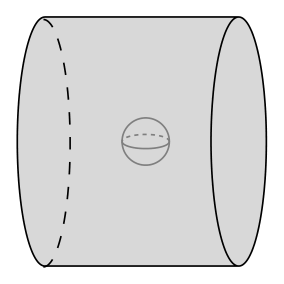
\includegraphics[width=0.10\textwidth]{p174_d1.png}}\quad;\quad
\text{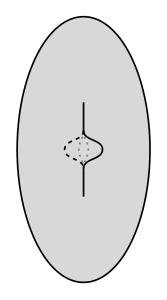
\includegraphics[width=0.055\textwidth]{p174_d2.png}}.
\end{equation}
形式上，当我们坍缩时间时，我们从
\begin{equation}\tag{10.249}
(C\times I)\setminus x\ \rightsquigarrow\ C\sqcup_{C\setminus x}C
\end{equation}
过渡。

回忆我们可以把局部算子看成平凡线缺陷的自同态。坍缩时间之后，这幅图告诉我们同一陈述的高维版本：\textbf{线算子是平凡曲面缺陷的自同态}。即考虑平凡曲面缺陷：
\begin{equation}\tag{10.250}
\{x\}\times I\times\R\subset C\times I\times\R.
\end{equation}
那么线缺陷 $\{x\}\times\{i\}$ 可以看成平凡曲面缺陷的一个自同态。要点是：当我们改为把线算子看成来自 $C\sqcup_{C\setminus x}C$ 时，它仍然是平凡曲面缺陷的自同态。

我们可以描述 $C\sqcup_{C\setminus x}C$ 上的 $G$-丛：
\begin{align}
\Bun_G\big(C\sqcup_{C\setminus x}C\big)&=\Bun_G(C)\times_{\Bun_G(C\setminus x)}\Bun_G(C)\tag{10.251}\\
&=\Big\{P_1,P_2\in\Bun_G(C),\ P_1|_{C\setminus x}\xrightarrow{\ \sim\ }P_2|_{C\setminus x}\Big\},\tag{10.252}
\end{align}
即这样的丛由 $C$ 上的一对丛以及在 $x$ 之外的同构组成。有一个 $G$-丛空间（即我们理论的场）的对应：
\begin{equation}\tag{10.253}
\begin{array}{ccc}
& \mathrm{Hecke}_x=\Bun_G\big(C\sqcup_{C\setminus x}C\big) &\\[4pt]
\swarrow & & \searrow\\[4pt]
\Bun_G(C) & & \Bun_G(C).
\end{array}
\end{equation}
于是我们可以把这个对应看成通过对 $\Bun_G$ 的任何线性化作推—拉来定义其上的算子。这就是我们解释线算子作用的方式。显式地
\begin{equation}\tag{10.254}
\mathcal{A}_G(C)=\Shv\big(\Bun_G(C)\big)
\end{equation}
（对某种拓扑的层概念），然后我们将用这个 Hecke 对应的推—拉在其上构造算子。

我们可以把从 $C$ 到 $C\sqcup_{C\setminus x}C$ 的过渡看成粘一个气泡：
\begin{equation}\tag{10.255}
D\sqcup_{D\setminus x}D\;=\;\text{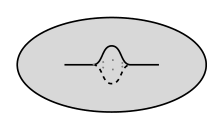
\includegraphics[width=0.075\textwidth]{p175_d3.png}}
\end{equation}
粘到 $C$ 上、沿 $x\in C$ 周围的某个圆盘 $D$：
\begin{equation}\tag{10.256}
C\sqcup_{C\setminus x}C=C\sqcup_D\big(D\sqcup_{D\setminus x}D\big)
\;=\;\text{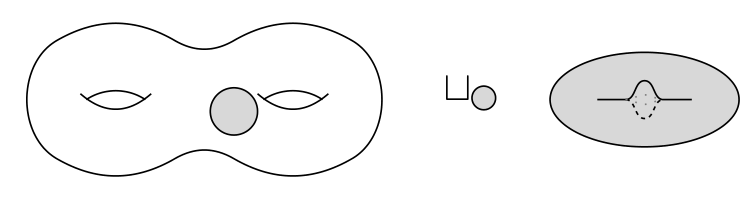
\includegraphics[width=0.22\textwidth]{p175_d4.png}}.
\end{equation}
用 $G$-丛来说，这意味着我们可以写：
\begin{align}
\mathrm{Hecke}_x&=\Bun_G\big(C\sqcup_{C\setminus x}C\big)\tag{10.257}\\
&=\Bun_G(C)\times_{\Bun_G(C\setminus x)}\Bun_G(C)\tag{10.258}\\
&=\Bun_G(C)\times_{\Bun_G(D)}\Big(\Bun_G(D)\times_{\Bun_G(D^{*})}\Bun_G(D)\Big).\tag{10.259}
\end{align}
即：与其把 $\mathrm{Hecke}_x$ 的元素描述为在 $x$ 之外带同构的一对 $G$-丛，我们可以把它们想成沿圆盘 $D$ 作修改的单个丛。

回忆 $\Bun_G(C,x)$ 是带“$x\in C$ 周围某个圆盘上的平凡化”的 $G$-丛空间。于是我们可以把 $\mathrm{Hecke}_x$ 重新写成：$\Bun_G(C,x)$ 与“圆盘上平凡 $G$-丛的所有修改”构成的空间的乘积，再模掉平凡化变换群 $G(\mathcal{O}_x)$：
\begin{equation}\tag{10.260}
\mathrm{Hecke}_x=\big(\Bun_G(C,x)\times\text{modifications}\big)\big/G(\mathcal{O}_x).
\end{equation}
这其实是我们已经见过的东西的一个版本，例如定理~5：
\begin{equation}\tag{10.261}
\Bun_G=G(F_x)\backslash\prod_{x\in C}^{\prime}G(K_x)/\prod_{x\in C}G(\mathcal{O}_x).
\end{equation}
当我们在 $x\in C$ 周围作平凡化时，我们玩同样的游戏，只是不模掉右边的一个因子：
\begin{equation}\tag{10.262}
\Bun_G(C,x)=G(F)\backslash\prod_{y}^{\prime}G(K_y)/\prod_{y\neq x}G(\mathcal{O}_y).
\end{equation}
于是这个空间带有整个圈群 $G(K_x)$ 的作用。所以我们有 $\Bun_G(C)$，它带有群 $G(\mathcal{O}_x)$ 的主丛：
\begin{equation}\tag{10.263}
\begin{array}{c}
\Bun_G(C,x)\\[2pt]
\downarrow{\scriptstyle G(\mathcal{O}_x)}\\[2pt]
\Bun_G(C)
\end{array}
\end{equation}
而全空间有大群 $G(K_x)$ 的作用。换言之，$\Bun_G(C)$ 是 $G(K_x)$-空间对子群 $G(\mathcal{O}_x)\subset G(K_x)$ 的商，而 Hecke 修改一般正是从这里来的。于是我们有：
\begin{equation}\tag{10.264}
\mathrm{Hecke}_x\simeq\big(\Bun_G(C,x)\times G(K_x)/G(\mathcal{O}_x)\big)\big/G(\mathcal{O}_x),
\end{equation}
即这是从主 $G(\mathcal{O})$-丛 $\Bun_G(C,x)$ 出发、在 $\Bun_G$ 上的相伴 $G(K)/G(\mathcal{O})$-丛。

所以我们有：
\begin{equation}\tag{10.265}
\begin{array}{ccc}
\Bun_G(C,x) & \longrightarrow & G(K_x)\\[4pt]
\downarrow{\scriptstyle G(\mathcal{O}_x)} & & \\[4pt]
\Bun_G(C) & &
\end{array}
\end{equation}
这给出 Hecke 群胚的作用：
\begin{align}
G(\mathcal{O}_x)\backslash G(K_x)/G(\mathcal{O}_x)&=\Bun_G\big(D\sqcup_{D\setminus x}D\big)\tag{10.266}\\
&=\text{$D$ 上丛的修改}\tag{10.267}\\
&=\Big\{P_1,P_2\in\Bun_G(D),\ P_1|_{D^{*}}\xrightarrow{\ \sim\ }P_2|_{D^{*}}\Big\}.\tag{10.268}
\end{align}

这一切的结论是如下。在物理图像中
\begin{equation}\tag{10.269}
\mathcal{A}_G\big(S^2\big)=\Shv\big(\Bun_G(S^2)\big)
\end{equation}
被线算子作用。在群论图像中，我们有这个 Hecke 东西的作用，即意大利饺上 $G$-丛的层：
\begin{equation}\tag{10.270}
\Shv\big(G(\mathcal{O})\backslash G(K)/G(\mathcal{O})\big)=
\Shv\Big(\Bun_G\big(\text{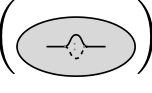
\includegraphics[width=0.07\textwidth]{p177_d1.png}}\big)\Big).
\end{equation}
但想法是：一旦我们给意大利饺填上足够的馅，这两者相距不远。

这就是\term{球 Hecke 范畴}{spherical Hecke category}的定义：
\begin{equation}\tag{10.271}
\Sph:=\Shv\big(G(\mathcal{O})\backslash G(K)/G(\mathcal{O})\big).
\end{equation}
这是几何 Langlands 纲领中的中心对象。它通过 Hecke 算子作用在 $\Shv(\Bun_G C)$ 上。所以我们看到了来自数论的阿黛尔描述，它说 $\Bun_G$ 有很多由对应实现的对称性：它不是群，但它是一个带群作用的空间的商。这正是我们得到这种由 Hecke 算子实现的剩余对称性的时候。然后我们可以把这些 Hecke 算子看成理论的线算子，而线算子是交换的。所以 $\Sph$ 是一个交换张量范畴，尽管 Hecke 代数/范畴一般并不交换。（原稿批注：move example?——此例是否移位待定。）

\begin{srcex}{70}（经典 Hecke 对应）
设 $V$ 是 $C$ 上秩 $n$ 的向量丛，$x\in C$。现在我们要“在 $x$ 处修改 $V$”。最容易的做法是看：
\begin{equation}\tag{10.272}
V(-x)=V\otimes\mathcal{O}(-x)\hookrightarrow V,
\end{equation}
它的截面定义为在 $x$ 处消失的 $V$ 的截面。这是我们在交换情形所做的，即给定线丛，这只是修改相应的除子。

下面是一个更有意思的修改。设 $W$ 是 $V|_x$ 的 $k$ 维子空间。那么我们可以修改 $W$ 得到 $V(-W)$，其截面由在 $x$ 处落在 $W$ 中的 $V$ 的截面给出，即：
\begin{equation}\tag{10.273}
\Gamma\big(V(-W)\big)=\big\{s\in\Gamma(V)\ \big|\ s|_x\in W\subset V|_x\big\}.
\end{equation}
这事实上是向量丛，且是 $V$ 的子丛。

这给出一种在一点处修改向量丛的方法，对任意子空间 $W$ 的选择，即在纤维的 $k$ 维子空间 Grassmann 簇中选一点：
\begin{equation}\tag{10.274}
W\in\Gr_k\big(V|_x\big).
\end{equation}
因此我们有一个对应：
\begin{equation}\tag{10.275}
\begin{array}{ccc}
& \mathrm{Hecke}^{k}_x &\\[4pt]
\swarrow & & \searrow\\[4pt]
\Bun_n(C) & & \Bun_n(C)
\end{array}
\end{equation}
其中
\begin{equation}\tag{10.276}
\mathrm{Hecke}^{k}_x=\text{“}\Gr_k(E|_x)\text{”}=\big\{(V,\,W\in\Gr_k(V|_x))\big\},
\end{equation}
而 $E$ 是万有丛。即这是一个以两种方式成为 $\Bun_n(C)$ 上 Grassmann 丛的对象，定义了上述对应：
\begin{equation}\tag{10.277}
\mathrm{Hecke}^{k}_x\;\rightsquigarrow\;
\big(V,\ W\in\Gr_k(V|_x)\big)\;\rightsquigarrow\;V(-W).
\end{equation}
\end{srcex}
于是 $\Bun_n(C)$ 回到自身的映射并没有那么多（若它是一个群我们可能会期待很多），但它是 $G$-空间的商，所以带有大量有意思的自对应；例如这里对任意非负整数 $k\le n$ 我们都得到一个。这些是基本的 Hecke 修改，它们将生成所有 Hecke 算子的格。

% [Tutor Note: 本节的记号是全书最密的：$F_x$ 是 $x$ 处的局部域、$\mathcal{O}_x$ 是其整数环、$K_x$ 是分式域（“圈群”$G(K_x)$ 即 $G$ 在局部域上的点）；$\prod'$ 表示阿黛尔意义下的受限乘积。(10.261) 中 $\Bun_G$ 与 $\Bun_G(C)$ 混用是原文写法（前者指整体模栈）。(10.262) 原文分母印作 $\prod_{y\ne x}G(\mathcal{O}_x)$，按意义应为 $G(\mathcal{O}_y)$，这是原稿的下标笔误，照译并指出。(10.273) 原文在两个集合之间漏印了关系符号，本译本按意义补为 $=$。最后要记住：几何 Langlands 的“自守侧”是 $\Shv(\Bun_G(C))$，“谱侧”由 Hecke 范畴 $\Sph$ 作用；Hecke 算子就是物理上的线算子，而线算子交换，这正是 $\Sph$ 虽是 Hecke 范畴却交换的原因。]

